% 若编译失败,且生成 .synctex(busy) 辅助文件,可能有两个原因:
% 1. 需要插入的图片不存在:Ctrl + F 搜索 'figure' 将这些代码注释/删除掉即可
% 2. 路径/文件名含中文或空格:更改路径/文件名即可

% --------------------- 文章宏包及相关设置 --------------------- %
% >> ------------------ 文章宏包及相关设置 ------------------ << %
% 设定文章类型与编码格式
\documentclass[UTF8]{report}		

% 本文的特殊宏定义
    \def\Im{\mathrm{Im\,}}
    \def\Re{\mathrm{Re\,}}
    \def\Arg{\mathrm{\,Arg\,}}
    \def\Ln{\mathrm{\,Ln\,}}
    \def\Arccos{\mathrm{\,Arccos\,}}
    \def\Arcsin{\mathrm{\,Arcsin\,}}
    \def\Arctan{\mathrm{\,Arctan\,}}
    \def\res{\mathrm{\,res\,}}
    \def\Res{\mathrm{\,Res\,}}
    \def\arcsinh{\mathrm{\,arcsinh\,}}
    \def\arccosh{\mathrm{\,arccosh\,}}
    \def\arctanh{\mathrm{\,arctanh\,}}
    \def\sgn{\mathrm{\,sgn\,}}

% 通用宏定义
    \def\N{\mathbb{N}}
    \def\F{\mathbb{F}}
    \def\Z{\mathbb{Z}}
    \def\Q{\mathbb{Q}}
    \def\R{\mathbb{R}}
    \def\C{\mathbb{C}}
    \def\T{\mathbb{T}}
    \def\S{\mathbb{S}}
    \def\A{\mathbb{A}}
    \def\I{\mathscr{I}}
    \def\d{\mathrm{d}}
    \def\p{\partial}



% 导入基本宏包
    \usepackage[UTF8]{ctex}     % 设置文档为中文语言
        \usepackage{hyperref}  % 宏包:自动生成超链接 (此宏包与标题中的数学环境冲突)
    \hypersetup{
        colorlinks=true,    % false:边框链接 ; true:彩色链接
        citecolor={blue},    % 文献引用颜色
        linkcolor={blue},   % 目录 (我们在目录处单独设置),公式,图表,脚注等内部链接颜色
        urlcolor={magenta},    % 网页 URL 链接颜色,包括 \href 中的 text
        % cyan 浅蓝色 
        % magenta 洋红色
        % yellow 黄色
        % black 黑色
        % white 白色
        % red 红色
        % green 绿色
        % blue 蓝色
        % gray 灰色
        % darkgray 深灰色
        % lightgray 浅灰色
        % brown 棕色
        % lime 石灰色
        % olive 橄榄色
        % orange 橙色
        % pink 粉红色
        % purple 紫色
        % teal 蓝绿色
        % violet 紫罗兰色
    }
    % \usepackage{docmute}    % 宏包:子文件导入时自动去除导言区,用于主/子文件的写作方式,\include{./51单片机笔记}即可。注:启用此宏包会导致.tex文件capacity受限。
    \usepackage{amsmath}    % 宏包:数学公式
    \usepackage{mathrsfs}   % 宏包:提供更多数学符号
    \usepackage{amssymb}    % 宏包:提供更多数学符号
    \usepackage{pifont}     % 宏包:提供了特殊符号和字体
    \usepackage{extarrows}  % 宏包:更多箭头符号
    \usepackage{multicol}   % 宏包:支持多栏 


% 文章页面margin设置
    \usepackage[a4paper]{geometry}
        \geometry{top=1in}  % 1 inch= 2.46 cm, 0.75 inch = 1.85 cm
        \geometry{bottom=1in}
        \geometry{left=0.75in}
        \geometry{right=0.75in}   % 设置上下左右页边距
        \geometry{marginparwidth=1.75cm}    % 设置边注距离(注释、标记等)

% 配置数学环境
    \usepackage{amsthm} % 宏包:数学环境配置
    % theorem-line 环境自定义
        \newtheoremstyle{MyLineTheoremStyle}% <name>
            {11pt}% <space above>
            {11pt}% <space below>
            {\kaishu}% <body font> 使用默认正文字体
            {}% <indent amount>
            {\bfseries}% <theorem head font> 设置标题项为加粗
            {:}% <punctuation after theorem head>
            {.5em}% <space after theorem head>
            {\textbf{#1}\thmnumber{#2}\ \ (\,\textbf{#3}\,)}% 设置标题内容顺序
        \theoremstyle{MyLineTheoremStyle} % 应用自定义的定理样式
        \newtheorem{LineTheorem}{Theorem.\,}
    % theorem-block 环境自定义
        \newtheoremstyle{MyBlockTheoremStyle}% <name>
            {11pt}% <space above>
            {11pt}% <space below>
            {\kaishu}% <body font> 使用默认正文字体
            {}% <indent amount>
            {\bfseries}% <theorem head font> 设置标题项为加粗
            {:\\ \indent}% <punctuation after theorem head>
            {.5em}% <space after theorem head>
            {\textbf{#1}\thmnumber{#2}\ \ (\,\textbf{#3}\,)}% 设置标题内容顺序
        \theoremstyle{MyBlockTheoremStyle} % 应用自定义的定理样式
        \newtheorem{BlockTheorem}[LineTheorem]{Theorem.\,} % 使用 LineTheorem 的计数器
    % definition 环境自定义
        \newtheoremstyle{MySubsubsectionStyle}% <name>
            {11pt}% <space above>
            {11pt}% <space below>
            {}% <body font> 使用默认正文字体
            {}% <indent amount>
            {\bfseries}% <theorem head font> 设置标题项为加粗
            {:\\ \indent}% <punctuation after theorem head>
            {0pt}% <space after theorem head>
            {\textbf{#3}}% 设置标题内容顺序
        \theoremstyle{MySubsubsectionStyle} % 应用自定义的定理样式
        \newtheorem{definition}{}

%宏包:有色文本框(proof环境)及其设置
    \usepackage[dvipsnames,svgnames]{xcolor}    %设置插入的文本框颜色
    \usepackage[strict]{changepage}     % 提供一个 adjustwidth 环境
    \usepackage{framed}     % 实现方框效果
        \definecolor{graybox_color}{rgb}{0.95,0.95,0.96} % 文本框颜色。修改此行中的 rgb 数值即可改变方框纹颜色,具体颜色的rgb数值可以在网站https://colordrop.io/ 中获得。(截止目前的尝试还没有成功过,感觉单位不一样)(找到喜欢的颜色,点击下方的小眼睛,找到rgb值,复制修改即可)
        \newenvironment{graybox}{%
        \def\FrameCommand{%
        \hspace{1pt}%
        {\color{gray}\small \vrule width 2pt}%
        {\color{graybox_color}\vrule width 4pt}%
        \colorbox{graybox_color}%
        }%
        \MakeFramed{\advance\hsize-\width\FrameRestore}%
        \noindent\hspace{-4.55pt}% disable indenting first paragraph
        \begin{adjustwidth}{}{7pt}%
        \vspace{2pt}\vspace{2pt}%
        }
        {%
        \vspace{2pt}\end{adjustwidth}\endMakeFramed%
        }

% 外源代码插入设置
    % matlab 代码插入设置
    \usepackage{matlab-prettifier}
        \lstset{style=Matlab-editor}    % 继承 matlab 代码高亮 , 此行不能删去
    \usepackage[most]{tcolorbox} % 引入tcolorbox包 
    \usepackage{listings} % 引入listings包
        \tcbuselibrary{listings, skins, breakable}
        \newfontfamily\codefont{Consolas} % 定义需要的 codefont 字体
        \lstdefinestyle{MatlabStyle_inc}{   % 插入代码的样式
            language=Matlab,
            basicstyle=\small\ttfamily\codefont,    % ttfamily 确保等宽 
            breakatwhitespace=false,
            breaklines=true,
            captionpos=b,
            keepspaces=true,
            numbers=left,
            numbersep=15pt,
            showspaces=false,
            showstringspaces=false,
            showtabs=false,
            tabsize=2,
            xleftmargin=15pt,   % 左边距
            %frame=single, % single 为包围式单线框
            frame=shadowbox,    % shadowbox 为带阴影包围式单线框效果
            %escapeinside=``,   % 允许在代码块中使用 LaTeX 命令 (此行无用)
            %frameround=tttt,    % tttt 表示四个角都是圆角
            framextopmargin=0pt,    % 边框上边距
            framexbottommargin=0pt, % 边框下边距
            framexleftmargin=5pt,   % 边框左边距
            framexrightmargin=5pt,  % 边框右边距
            rulesepcolor=\color{red!20!green!20!blue!20}, % 阴影框颜色设置
            %backgroundcolor=\color{blue!10}, % 背景颜色
        }
        \lstdefinestyle{MatlabStyle_src}{   % 插入代码的样式
            language=Matlab,
            basicstyle=\small\ttfamily\codefont,    % ttfamily 确保等宽 
            breakatwhitespace=false,
            breaklines=true,
            captionpos=b,
            keepspaces=true,
            numbers=left,
            numbersep=15pt,
            showspaces=false,
            showstringspaces=false,
            showtabs=false,
            tabsize=2,
        }
        \newtcblisting{matlablisting}{
            %arc=2pt,        % 圆角半径
            % 调整代码在 listing 中的位置以和引入文件时的格式相同
            top=0pt,
            bottom=0pt,
            left=-5pt,
            right=-5pt,
            listing only,   % 此句不能删去
            listing style=MatlabStyle_src,
            breakable,
            colback=white,   % 选一个合适的颜色
            colframe=black!0,   % 感叹号后跟不透明度 (为 0 时完全透明)
        }
        \lstset{
            style=MatlabStyle_inc,
        }

% table 支持
    \usepackage{booktabs}   % 宏包:三线表
    \usepackage{tabularray} % 宏包:表格排版
    \usepackage{longtable}  % 宏包:长表格

% figure 设置
    \usepackage{graphicx}  % 支持 jpg, png, eps, pdf 图片 
    \usepackage{subcaption} % 支持子图
    \usepackage{svg}       % 支持 svg 图片
        \svgsetup{
            % 指向 inkscape.exe 的路径
            inkscapeexe = C:/aa_MySame/inkscape/bin/inkscape.exe, 
            % 一定程度上修复导入后图片文字溢出几何图形的问题
            inkscapelatex = false                 
        }

% 图表进阶设置
    \usepackage{caption}    % 图注、表注
        \captionsetup[figure]{name=图}  
        \captionsetup[table]{name=表}
        \captionsetup{
            labelfont=bf, % 设置标签为粗体
            textfont=bf,  % 设置文本为粗体
            font=small  
        }
    \usepackage{float}     % 图表位置浮动设置 
    \usepackage{etoolbox} % 用于保证图注表注的数学字符为粗体
        \AtBeginEnvironment{figure}{\boldmath} % 图注中的数学字符为粗体
        \AtBeginEnvironment{table}{\boldmath}  % 表注中的数学字符为粗体
        \AtBeginEnvironment{tabular}{\unboldmath}   % 保证表格中的数学字符不受额外影响
% 圆圈序号自定义
    \newcommand*\circled[1]{\tikz[baseline=(char.base)]{\node[shape=circle,draw,inner sep=0.8pt, line width = 0.03em] (char) {\small \bfseries #1};}}   % TikZ solution

% 列表设置
    \usepackage{enumitem}   % 宏包:列表环境设置
        \setlist[enumerate]{
            label=(\arabic*) ,   % 设置序号样式为加粗的 (1) (2) (3)
            ref=\arabic*, % 如果需要引用列表项,这将决定引用格式(这里仍然使用数字)
            itemsep=0pt, parsep=0pt, topsep=0pt, partopsep=0pt, leftmargin=3.5em} 
        \setlist[itemize]{itemsep=0pt, parsep=0pt, topsep=0pt, partopsep=0pt, leftmargin=3.5em}
        \newlist{circledenum}{enumerate}{1} % 创建一个新的枚举环境  
        \setlist[circledenum,1]{  
            label=\protect\circled{\arabic*}, % 使用 \arabic* 来获取当前枚举计数器的值,并用 \circled 包装它  
            ref=\arabic*, % 如果需要引用列表项,这将决定引用格式(这里仍然使用数字)
            itemsep=0pt, parsep=0pt, topsep=0pt, partopsep=0pt, leftmargin=3.5em
        }  

% 其它设置
    % 脚注设置
    % 钩住脚注的内容,并将其设置为黑体
        \renewcommand\thefootnote{\ding{\numexpr171+\value{footnote}}}
    % 参考文献引用设置
        \bibliographystyle{unsrt}   % 设置参考文献引用格式为unsrt
        \newcommand{\upcite}[1]{\textsuperscript{\cite{#1}}}     % 自定义上角标式引用
    % 文章序言设置
        \newcommand{\cnabstractname}{序言}
        \newenvironment{cnabstract}{%
            \par\Large
            \noindent\mbox{}\hfill{\bfseries \cnabstractname}\hfill\mbox{}\par
            \vskip 2.5ex
            }{\par\vskip 2.5ex}

% 文章默认字体设置
    \usepackage{fontspec}   % 宏包:字体设置
        \setmainfont{SimSun}    % 设置中文字体为宋体字体
        \setCJKmainfont[AutoFakeBold=3]{SimSun} % 设置加粗字体为 SimSun 族,AutoFakeBold 可以调整字体粗细
        \setmainfont{Times New Roman} % 设置英文字体为Times New Roman

% 各级标题自定义设置
    \usepackage{titlesec}   
        % chapter 标题自定义设置
        \titleformat{\chapter}[hang]{\normalfont\huge\bfseries\centering\boldmath}{第\,\thechapter\,章}{20pt}{}
        \titlespacing*{\chapter}{0pt}{-20pt}{20pt} % 控制上下间距
        % section标题自定义设置 
        \titleformat{\section}[hang]{\normalfont\Large\bfseries\boldmath}{§\,\thesection\,}{8pt}{}
        % subsubsection标题自定义设置
        \titlespacing*{\subsubsection}{0pt}{3pt}{0pt} % 控制上下间距

% --------------------- 文章宏包及相关设置 --------------------- %
% >> ------------------ 文章宏包及相关设置 ------------------ << %

% ------------------------ 文章信息区 ------------------------ %
% ------------------------ 文章信息区 ------------------------ %
% 页眉页脚设置
    \usepackage{fancyhdr}   %宏包:页眉页脚设置
        \pagestyle{fancy}
        %\fancyhf{}\usepackage{lastpage} 
        %\cfoot{第 \thepage 页 / 共 \pageref{LastPage} 页}
        \cfoot{\thepage}
        \renewcommand\headrulewidth{1pt}
        \renewcommand\footrulewidth{0pt}
        \usepackage{fontawesome}    % 宏包:更多符号与图标 (用于插入 GitHub 图标等)
        \chead{Notes of Mathematical Physics Methods}     
        \rhead{\small dingyi233@mails.ucas.ac.cn}
        \lhead{\small
        \href{https://github.com/YiDingg/LatexNotes}{\color{black}\faGithub\ https://github.com/YiDingg/LatexNotes}
        }
%文档信息设置
    \title{数学物理方法笔记\\Notes of Mathematical Physics Methods}
    \author{丁毅\\ \footnotesize 中国科学院大学,北京 100049\\ Yi Ding \\ \footnotesize University of Chinese Academy of Sciences, Beijing 100049, China}
    \date{\footnotesize 2024.8 -- 2025.1}
% ------------------------ 文章信息区 ------------------------ %
% ------------------------ 文章信息区 ------------------------ %

% 开始编辑文章

\begin{document} 
\zihao{5}             % 设置全文字号大小, -4 为小四, 5 为五号

% ------------------------ 封面序言与目录 ------------------------ %
% >> --------------------- 封面序言与目录 --------------------- << %
% 封面
    \maketitle\newpage  
    \pagenumbering{Roman} % 页码为大写罗马数字
    \thispagestyle{fancy}   % 显示页码、页眉等

% 序言
\begin{cnabstract}\normalsize 
    本文为笔者本科时的“数学物理方法”课程笔记(Notes of Mathematical Physics Methods, 2024.9 - 2025.1)。读者可在笔者的个人网站 \href{https://yidingg.github.io/YiDingg/\#/Notes/Math/MathematicalPhysicsMathods}{https://yidingg.github.io/YiDingg/\#/Notes/Math/MathematicalPhysicsMathods} 上找到课程信息、教材、教辅和作业答案等相关资料。

    由于个人学识浅陋,认识有限,文中难免有不妥甚至错误之处,望读者不吝指正。读者可以将错误发送到我的邮箱 {\color{blue}\ dingyi233@mails.ucas.ac.cn},也可以到笔者的 \href{https://github.com/YiDingg/LatexNotes}{GitHub (https://github.com/YiDingg/LatexNotes)} 上提 issue,衷心感谢。
\end{cnabstract}

% 目录
    \setcounter{tocdepth}{2}                % 目录深度(为1时显示到section)
    \tableofcontents                        % 目录页
    \addcontentsline{toc}{chapter}{目录}    % 手动添加此页为目录
    \thispagestyle{fancy}                   % 显示页码、页眉等 

% 收尾工作
    \newpage    
    \pagenumbering{arabic} 


% >> --------------------- 封面序言与目录 --------------------- << %
% ------------------------ 封面序言与目录 ------------------------ %




\chapter{复数与复数运算}\thispagestyle{fancy} 
\section{预备知识}


\begin{definition}[复数定义]
    一个有序实数对 $(x,y)$ 称为复数如果其满足如下运算:
\begin{gather}
    \begin{aligned}
        &\text{加法}&&(x_1,y_1)+(x_2,y_2)=(x_1+x_2,y_1+y_2)\\
        &\text{乘法}&&(x_1,y_1)(x_2,y_2)=(x_1x_2-y_1y_2,x_1y_2+y_1x_2)
    \end{aligned}
\end{gather}
记作 $z = x + iy$,其中 $x = \R z$,$y = \I z$,$i^2 = 1$。

\end{definition}


\begin{definition}[相关概念] 
    下面是一些相关概念:
\begin{circledenum}
    \item 复数的三种表示:$z = x + iy = r(\cos \theta + i\sin \theta) =  re^{i\theta} = e^{\ln r + i\theta}$
    \item 模:$|z| = r =\sqrt{x^2+y^2}$
    \item 幅角:$\arg z = \theta \in [0, 2\pi)$ 称为幅角主值(或 $[-\pi, \pi)$),$\Arg z = \theta + 2k\pi$称为幅角补值,$k\in\Z$。
    \item 0 与 $\infty$:是两个特殊的复数,分别表示复平面中模为 0 和无穷大而幅角任意的“一个点”。在复平面的球表示中,$0$ 对应南极,$\infty$ 对应北极。
    \item 扩充复平面:称包含无穷远点 $\infty$ 的复平面 $\overline{\C} = \C \cup \{\infty\}$为扩充复平面。
    \item 共轭复数:$ z = x + iy, z^* = x - iy$
    \item 复数除法:设$z_1 = x_1 + iy_1, z_2 = x_2 + iy_2$,则:
    \begin{equation}
    \frac{z_1}{z_2}= \frac{x_1+\mathrm{i}y_1}{x_2+\mathrm{i}y_2}=\frac{(x_1+\mathrm{i}y_1)(x_2-\mathrm{i}y_2)}{(x_2+\mathrm{i}y_2)(x_2-\mathrm{i}y_2)} = \frac{1}{| z_2 |^2}\left[ (x_1x_2+y_1y_2) + \mathrm{i}(y_1x_2-x_1y_2) \right]
    \end{equation}
    用棣莫弗定理更易理解复数除法:设 $z_1 = r_1e^{i\theta_1}, z_2 = r_2e^{i\theta_2}$,则: 
    \begin{equation}
    \frac{z_1}{z_2} = \frac{r_1}{r_2}e^{i(\theta_1-\theta_2)}
    \end{equation}
    \item 复数乘法:$z_1z_2 = r_1r_2e^{i(\theta_1+\theta_2)}$
\end{circledenum}



\end{definition}


\section{复数序列}

\begin{definition}[相关概念]
    一个复数序列 $\{z_n\}$ 完全等价于两个实数序列 $\{x_n\}$ 和$\{y_n\}$
    \begin{circledenum}
        \item 聚点:给点复序列 $\{z_n\}$,若存在 $z \in \C$,使 $\forall\ \varepsilon >0$,恒有无穷多个$n$ 使得 $| z_n - z | < \varepsilon$则称$z$ 为序列$\{z_n\}$ 的一个聚点。
        {\par\color{gray}\small
        例如序列 $\{(-1)^{n+1}\frac n{n+1}\mid n \in \mathbb{N}_+\} =  \{\frac12,-\frac23,\frac34,-\frac45,\frac56,-\frac67,\cdots,(-1)^{n+1}\frac n{n+1},\cdots \}$ 有两个聚点 $1,-1$.
        \par}
        \item 有界 / 无界序列:序列 $\{z_n\}$ 称为有界的如果 $\exists\ M>0 \ \ \text{s.t.}\ \ | z_n | < M,\ \forall\ n \in \mathbb{N}_+$,否则称为无界的。
        \item 极限:称序列$\{z_n\}$收敛于$z \in \C$ 如果 $ \forall\ \varepsilon > 0,\ \exists\ N>0 \ \ \text{s.t.}\ \ | z - z_n | < \varepsilon, \forall\ n > N$ ,记作 $\displaystyle \lim_{n \rightarrow \infty} z_n = z $,否则称为发散序列。
        极限的必要条件是唯一聚点,无界序列不可能收敛
    \end{circledenum}
\end{definition}

\begin{LineTheorem}[Bolzano - Weierstrass 定理]\label{Bolzano - Weierstrass 定理}
任意有界序列至少有一个聚点。
\footnote{
    Theorem.\ref{Bolzano - Weierstrass 定理} 告诉我们有界序列必有聚点,事实上,在扩充复数域 $\overline{\C}$ 中,这对无界序列也成立($\infty$ 必为聚点),也即任意序列都必有聚点。}
\end{LineTheorem}

\begin{LineTheorem}[Cauchy判别法]\label{Cauchy判别法}
序列收敛的等价条件是:$\forall\ \varepsilon > 0, \exists\ N = N(\varepsilon) \ \ \text{s.t.}\ \ | z_{N+p} - z_N | < \varepsilon, \forall\ p \in \mathbb{N}_+$。
\end{LineTheorem}

\section{复变函数}


\begin{definition}[相关概念]
如下:
\begin{circledenum}
\item 点集:复平面内点的集合
\item 区域:复点集称为区域如果全部由内点组成,且具有连通性 
\footnote{连通性:集合中任意两点都可以用一条折线连接起来,且折线上的点全部属于此点集}
\item 单连通 / 多联通区域:区域称为单连通的如果在其内作任何简单闭合围道(自身不相交的闭合曲线),围道内的点都属于该区域,否则称为多联通区域(也称复联通区域)
{\par\color{gray}\small
例如,图 \ref{(a) (b) 构成区域,(c) 不构成区域} 中的 (a) 区域就属于单连通区域,而图 \ref{(a) (b) 构成区域,(c) 不构成区域} 中的(b)区域则为多连通区域。区域定义的条件之一就是仅包含内点,因此区域必是开集,$\overline{G} = G \cup \partial G$ 表示区域并上边界,称为闭域。
\par}
\item 边界:区域$G$ 的全体边界点构成其边界,记为 $\p G$
\item 边界方向:沿着区域的边界前进,区域恒保持在边界的左侧,则此走向称为边界的正向 
\end{circledenum}

\begin{figure}[H]\centering
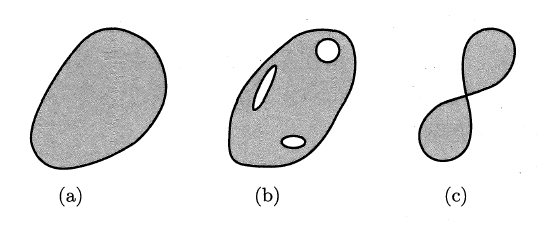
\includegraphics[width=0.45\textwidth]{assets/1,2/4d651e08624250e2b6a287f557fe1cf8.png}
\caption{\textbf{(a) (b) 构成区域,(c) 不构成区域}}\label{(a) (b) 构成区域,(c) 不构成区域}
\end{figure}
\end{definition}


\begin{definition}[复变函数]
复变函数 $f$ 是复数域子域 $G \subseteq \C$ 到复数域的映射,记作 $f:\ z \longmapsto \C$,或者 $f(z) = w,\ z \in G$。区域 $G$ 称为函数$f$  的定义域。事实上,复变函数等价于两个实变函数的有序组合。特别地,多值函数允许一个自变量对应多个函数值,我们在第二章会讨论。

\end{definition}

\section{无穷远点}

\begin{definition}[Riemann 球面]
如 图 \ref{Riemann 球面(复数球面)} ,过扩充的复平面$\overline{\C}$中的原点$(0,0)$作直径为 1 的球面,使之与$\overline{\C}$相切,切点称为南极 S,南极直径另一端称为北极 N。$\forall\ z \in \overline{\C}$,将它和复数球面的北极 N 相连,连线和球面有且仅有一个交点,因此存在一一对应关系。容易理解,$0$ 对应南极 S 而 $\infty$ 对应北极 N。

\begin{figure}[H]\centering
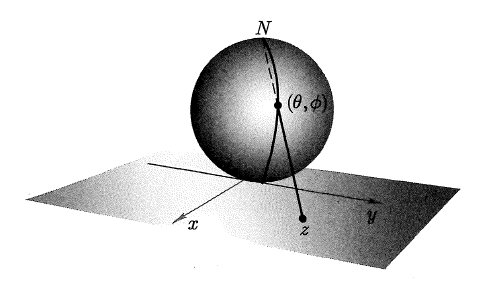
\includegraphics[width=0.40\textwidth]{assets/1,2/79ee2f440c28e683147e653d153efc72.png}
\caption{\textbf{Riemann 球面(复数球面)}}\label{Riemann 球面(复数球面)}
\end{figure}
\end{definition}

\section{复变函数可视化}
图 \ref{可视化1} (a) 是函数 $f(z) = z^2$ 的可视化,图 \ref{可视化1} (b) 是 $f(z) = z\cdot \Re z$ 的可视化。其中坐标 $(x,y)$ 对应 $z = x + iy$,箭头的长度代表 $| f(z) |$,方向代表 $\arg f(z)$。等高线表示模长相等。

\begin{figure}[H]\centering
\begin{subfigure}[t]{0.49\textwidth}\centering
    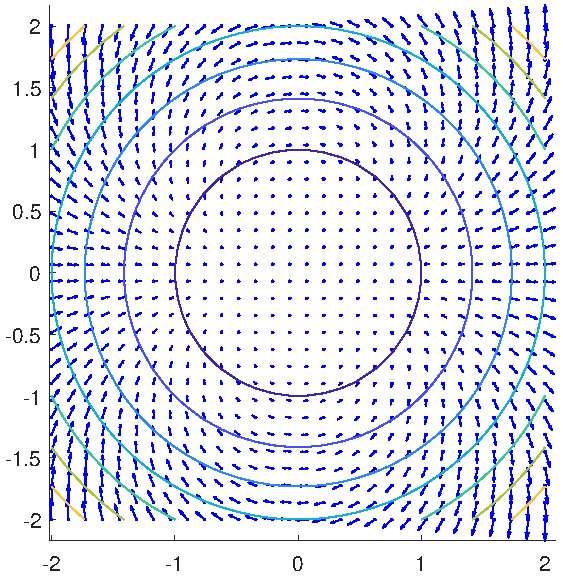
\includegraphics[height=220pt]{assets/1,2/z^2.pdf}
    \caption{ $f(z) = z^2$ }
\end{subfigure}\begin{subfigure}[t]{0.49\textwidth}\centering
    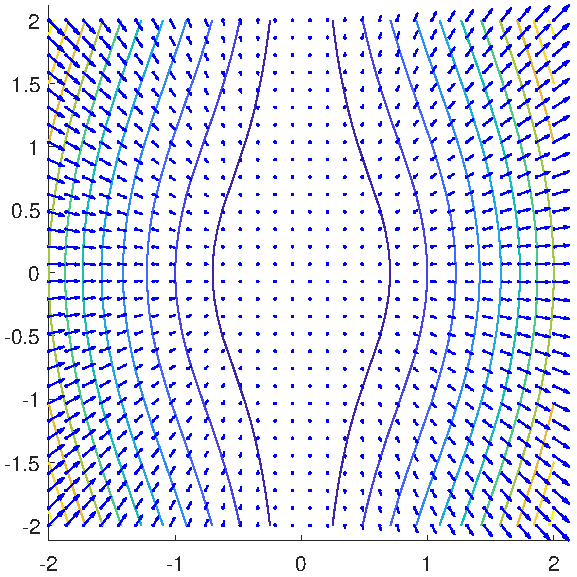
\includegraphics[height=220pt]{assets/1,2/zRez.pdf}
    \caption{ $f(z) = z\cdot \Re z$ }
\end{subfigure}
\caption{ 复变函数可视化 }\label{可视化1}
\end{figure}

图 \ref{可视化2} (a) 是 $f(z) = e^{iz}$,图 \ref{可视化2} (b) 是 $f(z) = cos(z)$。

\begin{figure}[H]\centering
    \begin{subfigure}[t]{0.49\textwidth}\centering
        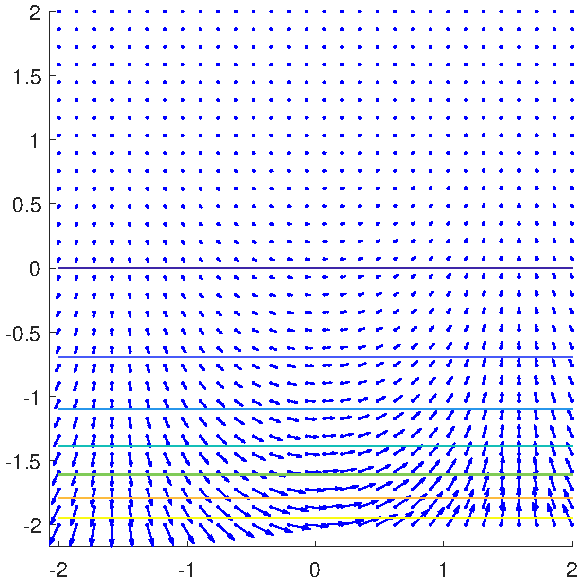
\includegraphics[height=220pt]{assets/1,2/e^(iz).pdf}
        \caption{ $f(z) = e^{iz}$ }
    \end{subfigure}\begin{subfigure}[t]{0.49\textwidth}\centering
        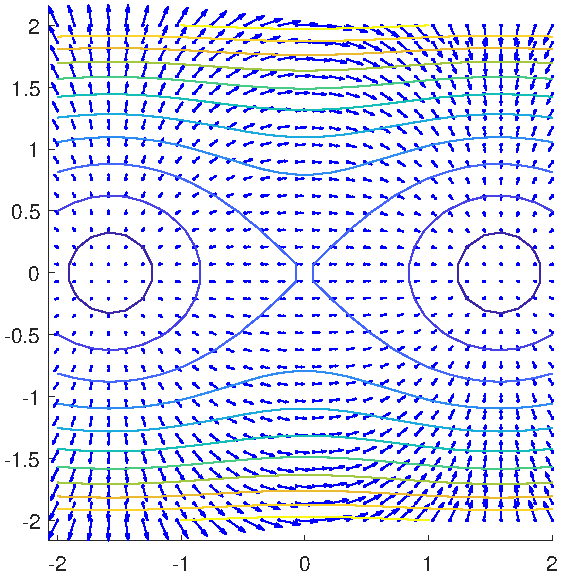
\includegraphics[height=220pt]{assets/1,2/cos(iz).pdf}
        \caption{ $f(z) = cos(z)$ }
    \end{subfigure}
    \caption{ 复变函数可视化 }\label{可视化2}
\end{figure}

\chapter{解析函数}\thispagestyle{fancy}

\section{复变函数的极限和连续}

\begin{definition}[极限]
设复变函数 $f(z)$ 在 $z_0$ 的空心邻域 $U^\circ_{\delta}(z_0)$ 中有定义\footnote{$z_0$ 的空心邻域是指以 $z_0$ 为圆心的环域 $0 < | z - z_0 | < \varepsilon$},
若 $\exists\ A \in \C $ 满足 $ \forall\ \varepsilon > 0,\ \exists\ \delta = \delta(\varepsilon)>0 \ \ \text{s.t.}\ \ | f(z) - A |<\varphi,\ \forall\ 0<| z - z_0 |<\delta $,则称 $z \to z_0$ 时 $f(z)$ 存在极限 $A$,记作:
\begin{equation}
\lim_{z \to z_0}f(z) = A
\end{equation} 
并且,设 $f(z) = u(z) + iv(z)$,$u,v$ 是 $\C$ 到 $\R$ 的函数,可以证明:
\begin{equation}
\lim_{z \to z_0}f(z) = \lim_{z \to z_0}u(z) + \mathrm{i}  \lim_{z \to z_0}v(z)
\end{equation} 
\end{definition}


\begin{definition}[连续]
设复变函数 $f(z)$ 在 $z_0$ 的邻域 $U_{\delta}(z_0)$ 中有定义,且 $ \lim_{z\to z_0}f(z) = f(z_0)$,则称 $f(z)$ 在 $z_0$ 处连续。

在有界必域 $\overline{G}$ 中连续的函数 $f(z)$ 具有两个重要性质:
\begin{circledenum}[leftmargin=4em]
\item  $ | f(z) | $ 在 $\overline{G}$ 中有界,并且上下界可取到
\item $f(x)$ 在 $\overline{G}$ 中一致连续,即 $| f(z_1) - f(z_2) | < \varepsilon, \forall\ | z_1 - z_2 | < \delta $
\end{circledenum}
\end{definition}


\section{可导与可微}



单值复变函数 $f(z)$ 在 $z_0$ 处可导如果 $\lim\frac{f(z + \Delta z) - f(z)}{\Delta z} = C \in \R$\footnote{这要求 $\Delta z$ 以任意方式趋于零,此极限都存在,类似二元函数的导数。}
,记为 $f'(z)$。


容易证明,高等数学中的各种求导公式都可以直接搬用到复变函数。

Cauchy-Riemann 条件是函数{\color{red} 可导的必要条件}:
\begin{gather}
\boxed{
    \frac{\partial u }{\partial x } = \frac{\partial v }{\partial y },\quad
    \frac{\partial u }{\partial y } = - \frac{\partial v }{\partial x }
}
\end{gather}
极坐标中的 C-R 条件:
\begin{equation}
\boxed{
    \frac{\partial u }{\partial r } = \frac{1}{r}\frac{\partial v }{\partial \phi },\quad \frac{\partial v }{\partial r } = - \frac{1}{r}\frac{\partial u }{\partial \phi }
}
\end{equation}


若存在 $A = A(z) \in \C \ \ \text{s.t.}\ \ \Delta f(z) = A(z) \cdot \Delta z + O(\Delta z)$,则称 $f(z)$ 在 $z_0$ 处可微,记作 $\mathrm{d} f = A \mathrm{d}z$,或 $\mathrm{d} f = A (\mathrm{d}x + i \mathrm{d}y)$

注意,与实变函数不同,在复变函数中,可导与可微是完全等价的:
\begin{equation}
{\color{red} f\ \text{可导}  \Longleftrightarrow   f \ \text{可微} }\Longleftrightarrow u,v\ \text{可导且满足 C-R 条件}  
\end{equation}

\section{解析函数}

\subsection{解析的概念与判定}
函数 $f$ 称为 $G$ 上的解析函数如果 $f$ 在区域 $G$ 内每一点都可导,又称为 $f$ 在 $G$ 上解析。


可以证明,函数 $f$ 在任意一点解析的充要条件是:
\begin{equation}
\text{$f$ 在点 $z \in \C$ 解析} \Longleftrightarrow \text{$f$ 在点 $z$ 可微且满足 Cauchy-Riemann 方程}
\end{equation}

在实际的操作中,我们常用下面定理来判断函数的解析性:
\begin{BlockTheorem}[解析函数判别法]\label{解析函数判别法}
设 $f(z) = u(x,y) + iv(x,y)$ 是区域 $G$ 上的单值复变函数,则:
\begin{gather}
\text{$u$ 和 $v$ 在 $G$ 上可微,且处处满足 C-R 条件} \Longleftrightarrow  \text{$f$ 在 $G$ 上可导}\Longleftrightarrow \text{ $f$ 在 $G$ 内解析} \\ 
\text{$u$ 和 $v$ 在 $G$ 上有连续一阶导,且处处满足 C-R 条件} \Longrightarrow \text{$f$ 在 $G$ 上可导}\Longleftrightarrow\text{$f$ 在 $G$ 内解析}
\end{gather}
\end{BlockTheorem}
{\par\color{gray}\small
对于第一行,$u$ 和 $v$ 在 $G$ 上可微并不能直接得到 $f$ 可微,例如 $u = 2x, v= -y$,还有加上 C-R 条件才能得到可微。对于第二行,$u$ 有一阶连续偏导 $\Longrightarrow $ $u$ 可微(多元实变函数的结论),后面同理
\par}


\subsection{已知实虚部求原函数}

在 $G$ 内解析的函数必满足 Cauchy-Riemann 方程(因为处处可导),因此只要知道实虚部其中之一,例如 $f(x,y) = u(x,y) + iv(x,y)$ 的实部 $u(x,y)$,就可以唯一地确定其虚部(可加减实常数),这是因为:
\begin{gather}
\mathrm{d} v = \frac{\partial v }{\partial x }\mathrm{d}x + \frac{\partial v }{\partial y } \mathrm{d}y = - \frac{\partial u}{\partial y } \mathrm{d}x + \frac{\partial u}{\partial x } \mathrm{d}y \\ \Longrightarrow
v(x,y) = \int \left( - \frac{\partial u}{\partial y } \mathrm{d}x + \frac{\partial u}{\partial x } \mathrm{d}y  \right)
\end{gather}


为求此原函数,设 $v(x,y) = g_1(x,y) + g_2(y)$,则:
\begin{gather}
\frac{\partial v }{\partial x} = \frac{\partial g_1 }{\partial x } 
\Longrightarrow 
g_1(x,y) = \int \frac{\partial v }{\partial x } \mathrm{d} x = \int (- \frac{\partial u }{\partial y }) \mathrm{d}x
\\ 
\frac{\partial v }{\partial y } = \frac{\partial g_1 }{\partial y } + \frac{\partial g_2 }{\partial y } \Longrightarrow 
g_2(y) = \int (\frac{\partial v }{\partial y } - \frac{\partial g_1 }{\partial y }) \mathrm{d}y = \int (\frac{\partial u }{\partial x } - \frac{\partial g_1 }{\partial y }) \mathrm{d}y 
\end{gather}
最后相加即得 $v(x,y)$。

这也就是说,先考虑 $\frac{\partial v }{\partial x }$ 对 $x$ 的积分,得到 $g_1(x,y)$,然后考虑 $\frac{\partial v }{\partial y }$,{\color{red} 将其含 $x$ 的项全部舍弃}(因为它们属于 $g_1$),再对 $y$ 作积分。{\color{red} 两积分结果相加即得 $v(x,y)$。}

特别地,当已知 $u(x,y)$ 和 $v(x,y)$ 时,欲求 $f(z)$ 的表达式(而不是 $f(x,y)$),只需直接令表达式 $u + iv$ 的 $(x,y) = (z,0)$,也即: 
\begin{equation}
\boxed{
    {f(z) = \left[u(x,y) + iv(x,y)\right]_{x = z, y=0} = u(z,0) + iv(z,0)}
}
\end{equation}
具体原因我们会在第五章“解析延拓”处讨论。

\subsection{实虚部关系可视化}
    解析函数实部与虚部之间的这种依赖关系,还可以形象地表现出来。在 $x-y$ 平面中,分别作出 $u(x,y)$ 和 $v(x,y)$ 的等高线图,在任意一点 $(x,y)$,由 Cauchy-Reimann 方程,两者方向矢量的内积为零:
    \begin{equation}
    \begin{bmatrix}
        \frac{\partial u }{\partial y } & - \frac{\partial u }{\partial x }
    \end{bmatrix}
    \cdot 
    \begin{bmatrix}
        \frac{\partial v }{\partial y } \\  -\frac{\partial v }{\partial x }
    \end{bmatrix}
    = \frac{\partial u }{\partial y }\frac{\partial v }{\partial y } + \frac{\partial u }{\partial x } \frac{\partial v }{\partial x } = 0
    \end{equation}
    因此两者的等高线图处处正交(表现为曲线处处正交)。
    % {\par\color{gray}\small
    % 例如 $f(z) = z^2$,则:
    % \begin{gather*}
    %     f(z) 
    %     = \frac{1}{z^2}
    %     = \frac{1}{(x^2-y^2) + (2xy) \mathrm{i} } 
    %     = \frac{x^2-y^2}{(x^2 + y^2)^2} + \frac{-2xy}{(x^2 +y^2)^2}  % \mathrm{i} \\ 
    %     \Longrightarrow u(x,y) = \frac{x^2-y^2}{(x^2 + y^2)^2} ,\ v(x,% y) = \frac{-2xy}{(x^2 +y^2)^2}
    % \end{gather*}
    % 它们的等高线图如图 ;
    % \par}
    
    {\par\color{gray}\small
    例如 $f(z) = z^2$,则:
    \begin{gather*}
        f(z) 
        = z^2
        = (x^2-y^2) + (2xy) \mathrm{i} 
        \Longrightarrow u(x,y) = x^2-y^2 ,\ v(x,y) = 2xy
    \end{gather*}
    它们的等高线图如图 \ref{解析函数 $f(z) = z^2$ 实虚部示意图} 所示:
    \begin{figure}[H]\centering
    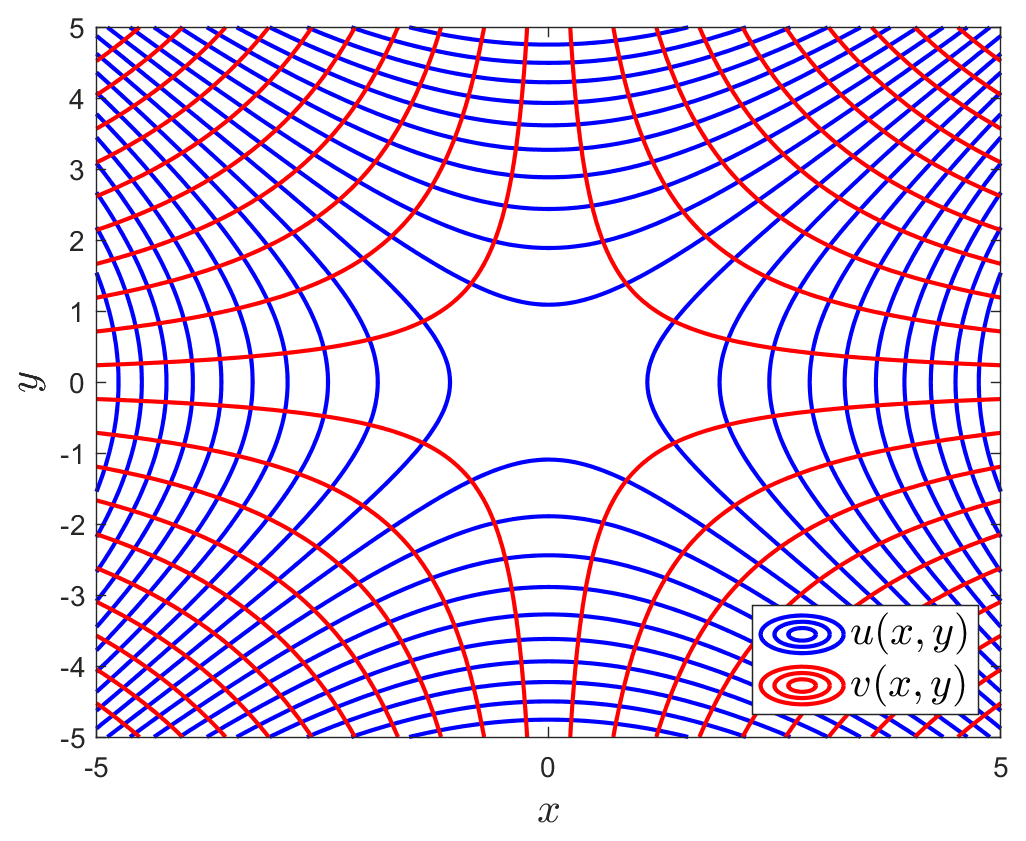
\includegraphics[width=0.3\textwidth]{assets/1,2/2024-08-28_10-23-23.png}
    \caption{\textbf{解析函数 $f(z) = z^2$ 实虚部示意图}}\label{解析函数 $f(z) = z^2$ 实虚部示意图}
    \end{figure}
    \par}
    
    之后我们会证明,解析函数 $f$ 的实部 $u(x,y)$ 和虚部 $v(x,y)$ 的二阶偏导一定存在且连续,并且满足二维 Laplace 方程\footnote{这样的函数 $f$ 称为调和函数},这表明解析函数的实部和虚部构成一对共轭的调和函数\footnote{共轭是因为满足 Cauchy-Riemann 方程}
    。
    \begin{equation}
        \Delta u = \Delta v = 0 \Longleftrightarrow
        \frac{\partial^{2}u}{\partial x^{2}}+\frac{\partial^{2}u}{\partial y^{2}}=\frac{\partial^{2}v}{\partial x^{2}}+\frac{\partial^{2}v}{\partial y^{2}}=0
    \end{equation}
    
    函数的解析性总是和给点区域联系在一起,有时也称函数在 $z_0$ 点解析,也即在邻域 $U_{\delta}(z_0)$ 内解析。讨论解析函数的各种特殊性质,就是复变函数论的中心课题。
    



\section{初等函数}

一些实初等函数推广到复数域时会有比较的特殊性质,下面进行讨论。



\begin{definition}[幂函数 $z^n$]
当 $n \in \N$ 时,$z^n$ 在 $\C$ 内解析,并且当 $n \in \N^*$时,$z^n$ 在 $\infty$ {\color{red} 不解析};当 $n \in -\N^*$ 时,$z^n$ 在 $z=0$ {\color{red} 不解析},在 $\overline{\C}\setminus \{0\}$ 内解析。
\end{definition}


\begin{definition}[指数函数 $e^z$]
复指数函数在 $\C$ 内解析,但在 $\infty$ 无意义,因为极限 $\lim_{z \to \infty}e^z$ 不存在
\begin{equation}
e^z = e^{x + \mathrm{i} y} = e^x(\cos y + \mathrm{i} \sin y)
\end{equation}
\end{definition}


\begin{definition}[三角函数 $\sin z,\ \cos z,\ ...$]
复三角函数是用复指数函数定义的,如下:
\begin{gather}
\boxed{
    \begin{aligned}
        \sin z
        =\frac{\mathrm{e}^{\mathrm{i}z}-\mathrm{e}^{-\mathrm{i}z}}{2i} 
        = \sin x \cosh y + {\color{red} i} \cos x \sinh y
        = \frac{1}{2{\color{red} i}}\cdot \left[ \left( e^y {\color{red} \,-\,} \frac{1}{e^y} \right)\cos x + {\color{red} i}\left( e^y +  \frac{1}{e^y}\right)\sin x \right]
        \\
        \cos z
        =\frac{\mathrm{e}^{\mathrm{i}z}+\mathrm{e}^{-\mathrm{i}z}}{2}
        = \cos x \cosh y - {\color{red} i} \sin x \sinh y
        = \frac{1}{2}\cdot \left[ \left(e^y + \frac{1}{e^y}  \right)\cos x {\color{red} \,- \,} {\color{red} i}\left( e^y {\color{red} \,-\,} \frac{1}{e^y} \right)\sin x \right]
    \end{aligned}
}
\end{gather}
$\sin z,\ \cos z$ 在 $\C$ 内解析,唯一奇点是 $z = \infty$。可以证明,实三角函数的各种恒等式对复三角函数仍成立(包括和差化积、万能公式等)。
\end{definition}


\begin{definition}[双曲函数 $\sinh z,\ \cosh z,\ ...$]
双曲函数也是通过复指数函数来定义的,如下
\begin{gather}
    \boxed{
    \begin{aligned}
        \sinh z
        = \frac{\mathrm{e}^{z}-\mathrm{e}^{-z}}{2} 
        = \sinh x \cos y + i \cosh x \sin y
        = \frac{1}{2}\cdot \left[ \left( \frac{1}{e^x} {\color{red} \,-\,} e^x \right)\cos y + \left( \frac{1}{e^x} + e^x \right)\sin y \right]
        \\
        \cosh z
        = \frac{\mathrm{e}^{z}+\mathrm{e}^{-z}}{2} 
        = \cosh x \cos y {\color{red} \,+\,} i \sinh x \sin y
        = \frac{1}{2}\cdot \left[ \left( \frac{1}{e^x} + e^x \right)\cos y + \left( \frac{1}{e^x} {\color{red} \,-\,} e^x \right)\sin y \right]
    \end{aligned}
    }
    \\
    \mathrm{sech}z=\frac{1}{\cosh z},\quad\cosh z=\frac{1}{\sinh z},\quad 
    \tanh z=\frac{\sinh z}{\cosh z},\quad \coth z=\frac{\cosh z}{\sinh z}
\end{gather}
由定义可知,双曲函数和三角函数能够互化:
\begin{equation}
    \sinh z=-\mathrm{i}\sin\mathrm{i}z,\quad\cosh z=\cos\mathrm{i}z,\quad\tanh z=-\mathrm{i}\tan\mathrm{i}z.
\end{equation}
通过上面的式子,我们也能很容易知道,在复数域上,三角函数不再是有界的函数了。另外注意导数公式:
\begin{equation}
    (\sinh z)'=\cosh z,\quad(\cosh z)'=\sinh z,\quad(\tanh z)'=\mathrm{sech}^2z
\end{equation}
其它结论:
\begin{gather}
    \cosh^{2}z-\sinh^{2}z=1, \quad1-\tanh^{2}z=\mathrm{sech}^{2}z \\ 
    \sinh\left(z_{1}\pm z_{2}\right)=\sinh z_{1}\cosh z_{2}\pm\cosh z_{1}\sinh z_{2}\\
    \cosh\left(z_{1}\pm z_{2}\right)=\cosh z_{1}\cosh z_{2}\pm\sinh z_{1}\sinh z_{2}
\end{gather}
\end{definition}

\section{解析函数的保角性(略)}
\section{多值函数}

\subsection{基本概念}

\begin{definition}[多值函数的概念]
$f$ 称为区域 $G \subseteq \C$ 上的多值函数如果 $\forall\ z \in G$ 存在多个 $w \in \C$ 使得 $f(z) = w_1 = w_2 = \cdots $。许多函数的逆运算都是多值函数。
\end{definition}

\begin{definition}[宗量、分支点]
考虑 $z-a$ 的开方 $w =\sqrt{z-a}$,设 $w = \rho_1 e^{\alpha}$ 而 $z-a = \rho_2e^{\theta}$,代入解得:
\begin{gather}
     w = \sqrt{| z-a |} e^{\frac{\theta}{2} + n\pi}, \quad n \in \Z \Longleftrightarrow 
     | w | = \sqrt{| z-a |},\quad \arg w = \frac{1}{2} \arg (z-a)
\end{gather}
$\omega $ 的多值性来源于 $z-a$ 幅角的多样性,我们把这样的量称为宗量\footnote{宗量通常不同于自变量.例如,多值函数 $\sqrt{z-a}$ 的宗量就是 $z-a$,多值函数号 $\sqrt[3]{(z - a)(z - b)}$ 的宗量就是$(z-a)(z-b)$。当然,也有宗量就是自变量的情形.例如多值函数 $\sqrt{z}$ 的宗量就是自变量 $z$。}(而不是自变量)。

为了进一步揭示多值函数 $w = \sqrt{z-a}$ 的性质,我们讨论“还原”与“不还原”。在 $z$ 复平面上依次画两个圆,如图 \ref{沿闭合曲线一周回到原处时} 左侧,第一个圆在点 $a$ 外,第二个圆包含了点 $a$。

对第一种情况,$z$ 沿路径 $C_1$ 逆时针旋转一圈后,由于 $a$ 在圆外,因此旋转前后的 $\arg (z-a)$ 不变,$\arg w = \frac{1}{2} \arg (z-a)$ 也不变,从而使得旋转前后 $w$ 也不变,称为 $w$ 值“还原”。对第二种情况,$z$ 沿路径 $C_2$ 逆时针旋转一圈后,由于 $a$ 在圆内,$\arg (z-a)$ 增加了 $2\pi$ 但 $\arg w = \frac{1}{2} \arg (z-a)$ 使得 $\arg w$ 仅增加 $\pi$,从而使得旋转前后 $w$ 未回到原点,称为 $w$ 值“不还原”。

因此,点 $a$ 对多值函数 $w =\sqrt{z-a}$ 有特殊意义,它是否位于简单闭合路径内就决定了当 $z$ 沿这个路径行进一周回到原处时,相应的 $w$ 值是否能还原。对于无法还原的点,我们称为\textbf{分支点}\footnote{分支点描述的是函数的多值性质,与函数的解析性无关}。也即,如果 $\exists\ r >0$,当 $z$ 沿圆周 $| z - z_0 | = r$ 绕一圈回到原处时,$w$ 不还原,且当 $r \mapsto 0$ 时,$w$ 始终不还原,这样的点 $z_0$ 就称为多值函数 $w(z)$ 的分支点。
{\par\color{gray}\small
例如,$z = a, \infty $ 是 $ f(z) = \sqrt{z - a} $ 的分支点,$z = a,b,c, \infty$ 是 $f(z) = \sqrt{(z-a)(z-b)(z-c)} $ 的分支点,$z = 0, \infty$ 是 $ f(z) = \Ln z = \ln | z | + i\Arg z$ 的分支点。
\par}
 


\begin{figure}[H]\centering
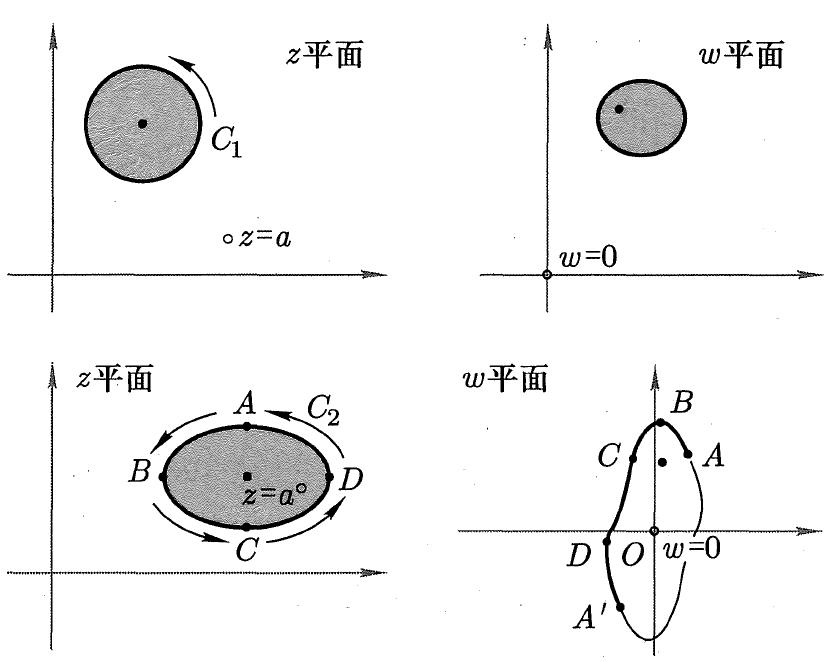
\includegraphics[width=0.55\textwidth]{assets/1,2/image (43).jpg}
\caption{\textbf{$z$ 沿闭合曲线一周回到原处时,$w = \sqrt{z-a}$ 值的不同变化}}\label{沿闭合曲线一周回到原处时}
\end{figure}
\end{definition}

\subsection{“有理”函数的分支点}
“有理”函数 $f(z)$: 
\begin{equation}
f(z) = \sqrt[k]{
    \frac{
        (z - z_{i_1})^{r_1}(z - z_{i_2})^{r_2} \cdot (z - z_{i_m})^{r_m}
    }{
        (z - z_{j_1})^{s_1}(z - z_{j_2})^{s_2} \cdot (z - z_{j_n})^{s_n}
    }
}
\end{equation}

\begin{enumerate}
\item 对 $a$: 若因式 $(z - a)^b$ 的幂指数 $b$ {\color{red} 不能}被根指数 $k$ 整除,即 $ b \ne 0\ (\text{mod}\  k) $,则 $a$ 为分支点,否则不是分支点。
\item 对 $\infty$: 若 $(\sum r_i - \sum s_i) \ne 0\ (\text{mod}\  k)$,则 $\infty$ 为分支点,否则不是分支点。
\end{enumerate}

\subsection{单值分支}
为了得到多值函数的单值分支,我们可以限制宗量的幅角范围(常通过“割线”来实现)。这样,宗量幅角范围的各个周期,给出多值函数的各个单值分支。另一种自然的方法是规定初始值和连续变化路线(移动路线)。

\subsection{常见多值函数}
最常见的多值函数是开根,在实际做题中,如果遇到开根 $\sqrt[n]{z} $,便是默认取 $z \in [0, 2\pi]$ 的单值分支。这里之所以取闭区间,是因为 $2\pi$ 可以取到,并且其值与 $0$ 不同。特别地,令 $z = x + iy = re^{i \theta},\ \theta \in [0, 2\pi]$,则 $\sqrt{z}$ 可以写为:
\begin{equation}
\boxed{
    \sqrt{z} =  \frac{1}{\sqrt{2}} \left( {\color{red} \text{sgn\,}(\pi -\theta)} \sqrt{| z | + x} + i \sqrt{| z | - x}  \right)
}
\end{equation}

对数函数和幂函数也是一种常见的多值函数:
\begin{gather}
    \ln z = \ln | z | + i\arg z,\quad
    \Ln z = \ln | z | + i\Arg z
\end{gather}

包括幂函数\footnote{在后文,除非特殊说明,都默认 $z^a$ 是取 $z \in [0, 2\pi]$ 时的单值分支,即 $z^a \mid_{z=1} = 1$}、三角函数在内的很多常见的多值函数都可以通过 $\Ln z$ 和根号来定义:
\begin{gather}
    \Arcsin z = \frac{1}{i}\Ln (iz + \sqrt{1-z^2} ),\quad
    \Arccos z = \frac{1}{i}\Ln (z + \sqrt{z^2 - 1} ) \\
    \Arctan z = \frac{1}{2i}\Ln(\frac{1+iz}{1-iz}) ,\quad
    z^\alpha = e^{\alpha \Ln z}= | z |^a \cdot e^{i\left(a \Arg z\right)},\  \alpha \in \C
\end{gather}


\section{部分复变函数可视化}

图 \ref{可视化3} 是 $f(z) = e^z$ 与 $f(z) = \cos (z)$ 的可视化,图 \ref{可视化4}\footnote{图 \ref{可视化3} 和图 \ref{可视化4} 源码见附录 \ref{可视化34 源码}} 是多值函数 $f(z) = \sqrt{z}$ 和 $f(z) = \Ln z$ 的单值分支的可视化,图中等高线表示模长相等。

\begin{figure}[H]\centering
\begin{subfigure}[t]{0.49\textwidth}\centering
    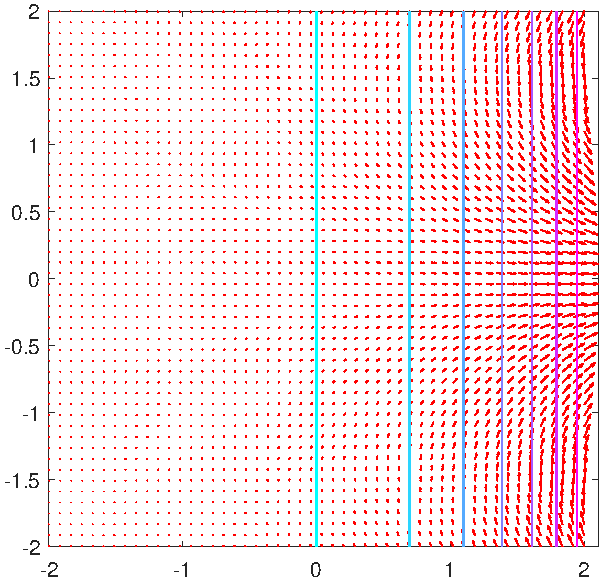
\includegraphics[height=205pt]{assets/1,2/e^z.pdf}
    \caption{ $\boldsymbol{f(z) = e^z}$ }
\end{subfigure}\begin{subfigure}[t]{0.49\textwidth}\centering
    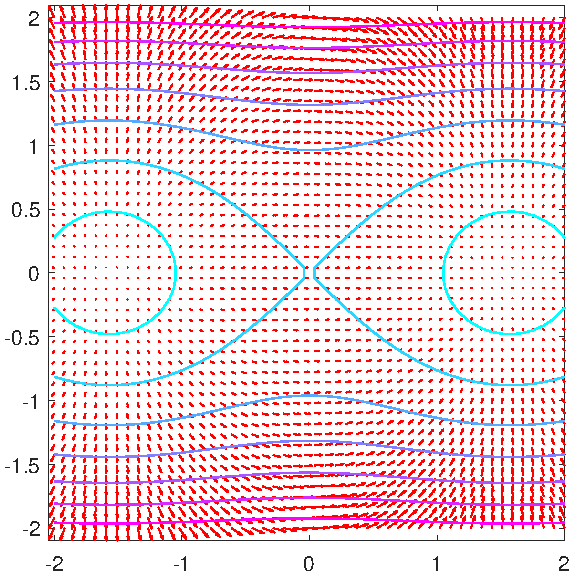
\includegraphics[height=205pt]{assets/1,2/cos z.pdf}
    \caption{ $\boldsymbol{f(z) = \cos (z)}$ }
\end{subfigure}
\caption{ 单值复变函数可视化 }\label{可视化3}
\end{figure}


\begin{figure}[H]\centering
    \begin{subfigure}[t]{0.49\textwidth}\centering
        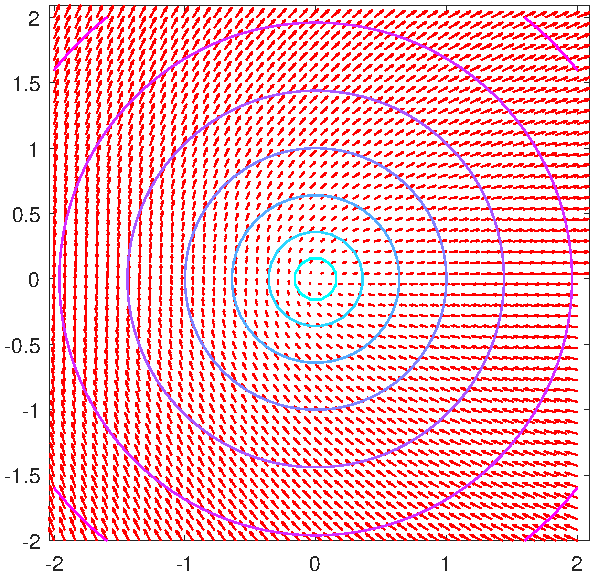
\includegraphics[height=205pt]{assets/1,2/sqrt z.pdf}
        \caption{ $\boldsymbol{f(z) = \sqrt{z} },\ \boldsymbol{\arg z \in [0, 2\pi]}$ 单值分支 }
    \end{subfigure}\begin{subfigure}[t]{0.49\textwidth}\centering
        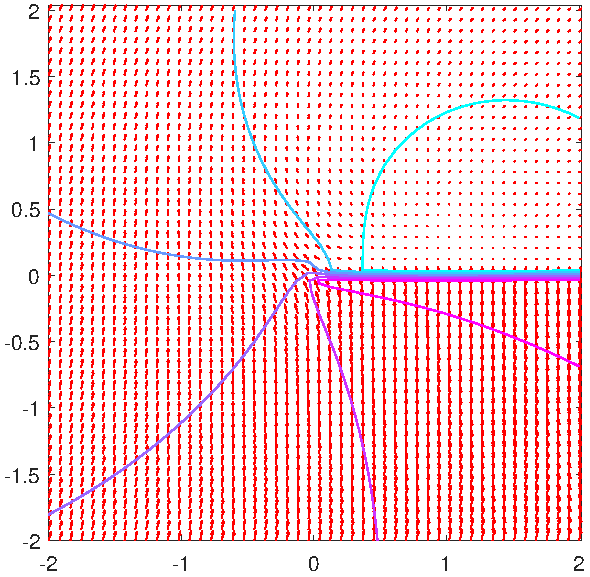
\includegraphics[height=205pt]{assets/1,2/ln z.pdf}
        \caption{ $\boldsymbol{f(z) = \Ln z},\ \boldsymbol{\arg z \in [0, 2\pi]}$ 单值分支  }
    \end{subfigure}
    \caption{ 多值复变函数可视化 }\label{可视化4}
\end{figure}

\section{常见函数总结}

三角函数及其反函数:
\begin{align}
    \sin z
    &=\frac{\mathrm{e}^{\mathrm{i}z}-\mathrm{e}^{-\mathrm{i}z}}{2i} 
    = \sin x \cosh y + i \cos x \sinh y
    \\
    \cos z
    &=\frac{\mathrm{e}^{\mathrm{i}z}+\mathrm{e}^{-\mathrm{i}z}}{2}
    = \cos x \cosh y - i \sin x \sinh y
    \\ 
    \tan z &= \frac{\sin z}{\cos z} = -i \cdot \frac{e^{iz} - e^{-iz}}{e^{iz} + e^{-iz}} = -i \cdot \frac{e^{2iz} - 1}{e^{2iz} + 1}
\end{align}
\begin{align}
    \arcsin z &= -i \cdot \ln \left(iz + \sqrt{1 - z^2}\right) \\ 
    \arccos z &= -i \cdot \ln \left(z + \sqrt{z^2 - 1}\right) \\
    \arctan z &= -\frac{i}{2} \ln \left(\frac{1 + iz}{1 - iz}\right)
\end{align}

双曲函数及其反函数:
\begin{align}
\sinh z &= \frac{e^z - e^{-z}}{2} = \sinh x \cos y + i \cosh x \sin y\\ 
\cosh z &= \frac{e^z + e^{-z}}{2} = \cosh x \cos y + i \sinh x \sin y\\ 
\tanh z &= \frac{\sinh z}{\cosh z} = \frac{e^z - e^{-z}}{e^{z} + e^{-z}} = \frac{e^{2z} - 1}{e^{2z} + 1}
\end{align}
\begin{align}
    \arcsinh z &= \ln \left(z + \sqrt{z^2 + 1} \right) \\ 
    \arccosh z &= \ln \left(z + \sqrt{z^2 - 1} \right) \\ 
    \arctanh z &= \frac{1}{2}\cdot \ln \left(\frac{1 + z}{1 - z}\right)
\end{align}

根号函数:
\begin{equation}
    \sqrt{z} = \frac{1}{\sqrt{2}} \left( \text{sgn}(\pi -\theta) \sqrt{| z | + x} + i \sqrt{| z | - x}  \right),\quad 
    \sgn x = \begin{cases}
        -1, & x < 0 \\
        1, & x > 0 \\ 
        0, & x = 0  
    \end{cases}
\end{equation}

\chapter{复变积分}

\section{复变积分的概念}
复变积分是 $\C$ 上的线积分,沿某条路径,由点 A 至点 B 的复变积分定义为:
\begin{equation}
I = \lim_{\max | \Delta z_i \to 0|}\sum_{i=1}^{n} f(\xi_i)\Delta z_i = \int_{C_{AB}} f(z) \mathrm{d}z
\end{equation}
如果路径是闭合的,也常称为积分围道。一个复变积分实际上是两个实变线积分的线性组合,因此,若 $C$ 是分段光滑曲线,且 $f(z)$ 在路径 $C$ 上连续,则复变积分一定存在。
\begin{equation}
\int_{C}f(z) \mathrm{d}z = \int_{C}(u \mathrm{d}x - v \mathrm{d}y) + i \int_{C}( v \mathrm{d}x + u \mathrm{d}y)
\end{equation}

\section{Cauchy 定理}

\subsection{Cauchy-Goursat 定理}

\begin{BlockTheorem}[Cauchy 定理\footnote{也称 Cauchy-Goursat 定理}]\label{Cauchy 定理}
若 $f(z)$ 在{\color{red} 有界}开域 $G$ 上单值解析,在 $\partial G$ 上连续\footnote{有的教材称上述两个条件是“在闭域 $\overline{G}$ 中解析”,详见附录 \ref{在闭域上解析}},则:
\begin{gather}
\oint_{\partial G} f(z) \mathrm{d}z = 0
\end{gather}
对单连通区域,$\partial G$ 即为外围边界线(沿逆时针);对多连通区域,外围边界线沿逆时针积分,内部边界线沿顺时针积分\footnote{始终保持区域在自身左侧的走向称为正向。}。
\end{BlockTheorem}

\subsection{Cauchy 定理的推广}

\begin{BlockTheorem}[Cauchy 定理推广1]\label{Cauchy 定理推广1}
连续函数 $f$ 在有界复连通区域 $G$ 上单值解析,则:
\begin{equation}
\oint_{C_0} f(z) \mathrm{d}z = \sum_{i=1}^{i=n} \oint_{C_i^{(-)}} f(z) \mathrm{d}z
\end{equation}
路径上的负号表示路径沿反相,在这里即沿逆时针。也就是所有路径(包括 $C_0$)都沿逆时针。
\end{BlockTheorem}

\begin{BlockTheorem}[Cauchy 定理推广2]\label{Cauchy 定理推广2}
    连续函数 $f$ 在有界单连通区域 $G$ 上单值解析,则:
    \begin{equation}
    \text{$\oint_C f(z)\mathrm{d}z,\ C \subset G$ 与路径无关,也即 $f(z)$ 存在原函数}
    \end{equation}
\end{BlockTheorem}

\begin{BlockTheorem}[Cauchy 定理推广3]\label{Cauchy 定理推广3}
    $C$ 为 $G$ 的边界,任取简单闭合曲线 $C' \subset G$,若连续函数 $f(z)$ 在构成的新有界复连通区域上解析,则:
    \begin{equation}
        \oint_{C} f(z) \mathrm{d}z = \oint_{C'} f(z) \mathrm{d}z
    \end{equation}
\end{BlockTheorem}

\subsection{Cauchy 定理推论}

\begin{BlockTheorem}[Morera 定理]\label{Morera 定理}
设 $f$ 在闭域 $\overline{G} $ 中连续,且对 $G$ 中任意闭合围道 $C$,都有 $\oint_{C} f(z) \mathrm{d}z = 0$,则 $f$ 在 $G$ 中解析。结合 Cauchy 定理的正表述,也即:
\begin{equation}
f(z) \ \text{在 $\overline{G} $ 内解析} \Longleftrightarrow  \oint_{C} f(z) \mathrm{d}z = 0,\ \forall\ C \subset \overline{G}  \Longleftrightarrow  \ \text{积分} \int_{z_1}^{z_2} f(z) \mathrm{d}z \ \text{与路径无关},\ z_1, z_2 \in \overline{G} 
\end{equation}

Morera 定理可以理解为 Cauchy 定理的逆定理,用于判别函数在某区域上的解析性。
\end{BlockTheorem}

\begin{LineTheorem}[最大模原理]\label{最大模原理}
    设 $f(z)$ 在 $\overline{G}$ 中解析,则模 $| f(z) |$ 的最大值一定在边界 $\partial G$ 上。
\end{LineTheorem}


\begin{BlockTheorem}[Cauchy 不等式]\label{Cauchy 不等式}
设函数 $f$ 在 $\overline{G}$ 中解析,则有不等式:
\begin{equation}
\left| f^{(n)}(z) \right| \leqslant \frac{n!}{2 \pi d^{n+1}}\cdot Ml ,\quad n = 0, 1, 2, ...
\end{equation}

其中 $M = \sup \{ | f(z) |,\ z \in \partial G \}$ 是 $| f(z) |$ 在边界取值的上界,$l = \int_{\partial G} \mathrm{d}s$ 是边界 $\partial G$ 的长度,$d = \inf \{ \rho(z, \partial G) \}$ 是 $z$ 点到边界 $\partial G$ 的距离(距离即为下界)。事实上,由于 $\overline{G}$ 是闭域,这里的上界、下界均可取到,因此分别是最大值、最小值。

特别地,当边界是以 $z$ 为圆心,$R$ 为半径的圆时,不等式变为:
\begin{equation}
\left| f^{(n)}(z) \right| \leqslant \frac{n! M}{ R^{n}} ,\quad n = 0, 1, 2, ...
\end{equation}
\end{BlockTheorem}

\begin{LineTheorem}[Liouville 定理]\label{Liouville 定理}
若 $f(z)$ 在全平面上解析,且 $\displaystyle \lim_{z \to \infty} | f(z) | < \infty$,则 $f(z)$ 是常数函数。更优雅的说法是:“在全平面上解析的有界复变函数都是常数函数”。
\end{LineTheorem}

\begin{BlockTheorem}[均值定理]\label{均值定理}
设 $f(z)$ 在 $\overline{G}$ 内解析,则 $f$ 在 $G$ 内任意一点 $z_0$ 的函数值是它在圆周上取值的算术平均:
\begin{equation}
f(z_0) = \frac{1}{2\pi} \int_{0}^{2\pi} f(z_0 + R e^{i\theta}) \mathrm{d}\theta
\end{equation} 
其中 $R$ 是以 $z_0$ 为圆心,位于 $\overline{G}$ 内的任一圆周的半径。注意积分前的系数是 $\frac{1}{2\pi}$ 而不是 $\frac{1}{2\pi i}$。
\end{BlockTheorem}




\section{圆弧定理}
\begin{BlockTheorem}[小圆弧定理]\label{小圆弧定理}
若 $f(z)$ 在 $a$ 的空心邻域 $U_{\delta}^\circ(a)$ 上连续,且在 $\arg (z - a) \in [\theta_1,\ \theta_2]$ 时,$(z-a)f(z)$ 一致收敛于 $k$($| z -a |\to 0$),则:
\begin{equation}
\lim_{\delta \to 0} \int_{C_\delta} f(z)\mathrm{d}z = ik(\theta_2 - \theta_1)
\end{equation}
其中 $C_\delta$ 是以 $a$ 为圆心,$\delta$ 为半径,张角为 $\theta_2 - \theta_1$ 的小圆弧。
\end{BlockTheorem}

\begin{BlockTheorem}[大圆弧定理]\label{大圆弧定理}
    若 $f(z)$ 在 $\infty$ 的空心邻域 $U_{\delta}^\circ(\infty)$ 上连续,且在 $\arg (z - a) \in [\theta_1,\ \theta_2]$ 时,$(z-a)f(z)$ 一致收敛于 $k$($| z - a| \to \infty$),则:
    \begin{equation}
    \lim_{R \to \infty} \int_{C_R} f(z)\mathrm{d}z = ik(\theta_2 - \theta_1)
    \end{equation}
    其中 $C_R$ 是以 $a$ 为圆心,$R$ 为半径,张角为 $\theta_2 - \theta_1$ 的大圆弧。
    \end{BlockTheorem}

\section{Cauchy 积分公式}

\begin{BlockTheorem}[Cauchy 积分公式]\label{n 阶导数 Cauchy 积分公式}

若 $f(z)$ 在 $\overline{G} $ 中解析\footnote{解析域一定是开集,为什么这里会说在闭域上解析?详见附录 \ref{在闭域上解析}} ,则 $f(z)$ 在 $G$ 上有任意阶导数,且它们都是 $\overline{G} $ 上的解析函数。
\begin{equation}
f^{(n)}(z) = \frac{n !}{2\pi i}\oint_{\partial G} \frac{f(\zeta)}{(\zeta - z)^{n+1}} \mathrm{d} \zeta,\quad \forall\ z \in G
\end{equation} 
特别地,当 $n = 0$ 时,得到 Cauchy 积分公式\footnote{事实上是由 $n = 0$ 和归纳法证明的 n 阶导数 Cauchy 积分公式}: 
\begin{equation}
    f(z) = \frac{1}{2\pi i}\oint_{\partial G} \frac{f(\zeta)}{(\zeta - z)} \mathrm{d} \zeta,\quad \forall\ z \in G
\end{equation}
闭域 $\overline{G}$ 可以是复联通区域,积分路径仍沿正向,即内部顺时针,最外围逆时针。
\end{BlockTheorem}

\begin{BlockTheorem}[Cauchy 定理的推广]\label{Cauchy 定理的推广}
在计算回路积分时,Theorem.\ref{n 阶导数 Cauchy 积分公式} 使用起来不太方便,由小圆弧定理和 Cauchy 定理,我们可以证明下面命题,方便我们使用。

若 $f(z)$ 在 $\overline{G}$ 上有唯一奇点 $z = a$,且 $(z - a)^n f(z)$ 在  $\overline{G}$ 上解析,则:
\begin{equation}
I  = \oint_{\partial G} f(z) \mathrm{d}z = 2 \pi i \cdot \frac{1}{({\color{red} n-1})!} \left[(z - a)^{n} f(z) \right]^{({\color{red} n-1})}_{z = a}
\end{equation}
特别地,当 $n = 1$ 时,得到 Cauchy 积分公式。当 $n = 1$ 时,$z = a$ 可能是可去奇点,此时 $z = a$ 是指 $\lim_{z \to a}$。
\end{BlockTheorem}

\begin{BlockTheorem}[无界区域上的 Cauchy 积分公式]\label{无界区域上的 Cauchy 积分公式}

若 $f(z)$ 在 $ \C \setminus \overline{G} $ 中解析,则 $f(z)$ 在 $\C \setminus \overline{G}$ 上有任意阶导数,且它们都是 $\C \setminus \overline{G} $ 上的解析函数。
\begin{equation}
f^{(n)}(z) = \frac{n !}{2\pi i}\oint_{\partial G} \frac{f(\zeta)}{(\zeta - z)^{n+1}} \mathrm{d} \zeta,\quad \forall\ z \in\C \setminus \overline{G},\ n = 0,1,2,...
\end{equation} 

\end{BlockTheorem}

\section{Cauchy 型积分与含参量积分的解析性}

\begin{BlockTheorem}[Cauchy 型积分]\label{Cauchy 型积分}

设函数 $\phi$ 在分段光滑曲线 $L \in \C$ 上连续($L$ 可闭合或不闭合),则下面函数在 $\C \setminus L$ 上解析,在全平面上连续:
\begin{equation}
f (z) = 
\begin{cases}
    \phi(z) &, z \in L \\
    \displaystyle \frac{1}{2\pi i}\oint_{L} \frac{\phi(\zeta)}{\zeta - z} \mathrm{d} \zeta &, z \in \C \setminus L \\ 
\end{cases}
\end{equation}
且它在 $\C \setminus L$ 上的导数可由 Cauchy 积分公式得到:
\begin{equation}
f^{(n)}(z) = \frac{n !}{2\pi i}\oint_{L} \frac{\phi(\zeta)}{(\zeta - z)^{n+1}} \mathrm{d} \zeta,\quad \forall\ z \in \C \setminus L, n = 1,2,3,...
\end{equation}

%且 $f$ 在 $ G \subseteq \C \setminus L$ 上解析,则 $f$ 在 $G$ 内的值及其导数值被唯一确定:
%\begin{gather}
%f(z) = \frac{1}{2\pi i}\oint_{L} \frac{f(\zeta)}{\zeta - z} \mathrm{d} \zeta,\quad \forall\ z \in G \\ 
%f^{(n)}(z) = \frac{n !}{2\pi i}\oint_{L} \frac{f(\zeta)}{(\zeta - z)^{n+1}} \mathrm{d} \zeta,\quad \forall\ z \in G, n = 1,2,3,...
%\end{gather}
%{\par\color{gray}\small
%注:上面的定理事实上是 Cauchy 型积分 + 补充定义得来。为保持定理的易用性,我们直接将其称为 Cauchy 积分公式。定理的推广过程是: Cauchy 积分公式,解析函数的高阶导数,无界区域上的 Cauchy 积分公式,无界区域上的解析函数高阶导数,Cauchy 型积分。详见参考文献 \cite{数学物理方法} 的 Page 40-42.
%\par}
\end{BlockTheorem}

\begin{BlockTheorem}[含参量积分的解析性]\label{含参量积分的解析性}
设含参函数 $f = f(t,z)$ 分别对 $t\in L$ 和 $z\in \overline{G} $ 连续\footnote{这与在 $ L \times \overline{G}$ 上连续不同。}(对两个变量都连续),其中 $\overline{G} $ 是有界闭域。且 $\forall\ t \in L$,$f(t,z)$ 是 $\overline{G}$ 上的单值解析函数,则函数 $\displaystyle F(z) = \int_{L} f(t,z) \mathrm{d}t$
在 $G$ 内解析,且 $\displaystyle F'(z) =  \int_{L} \frac{\partial f(t,z) }{\partial z } \mathrm{d}t$。
\end{BlockTheorem}

\section{Poisson 公式}

Cauchy 积分公式告诉我们,对于在 $\overline{G} $ 上解析的函数 $f(z)$,函数在 $\overline{G} $ 内任意一条曲线上的值(可以是边界 $\partial G$)就完全唯一地决定了 $f$ 在 $G$ 内任意一点的值。特别地,当 $ G = \C$ 时,若已知 $f$ 在 $\C$ 内任意一条(分段光滑)曲线 $L$ 上的值,都可求出 $f$ 在全平面的值。

\begin{BlockTheorem}[上半平面 Poisson 公式]\label{上半平面 Poisson 公式}
如果 $f(z)$ 在上半平面解析,且 $\lim_{z \to \infty} f(z) = 0$,则可依据它(或者它的实部或虚部)在实轴上的值,求出它在整个上半平面的值:
\begin{gather}
    \begin{aligned}
        \text{已知}\ f(z),& z \in \R\ \text{:}  \quad \quad \quad 
        && f(z) 
        = \frac{1}{2 \pi i} \int_{-\infty}^{+ \infty} \frac{f(\xi)}{\xi - z} \mathrm{d}\xi \\ 
        &= \frac{y}{\pi} \int_{-\infty}^{+ \infty} \frac{f(\xi)}{(\xi - x)^2 + y^2} \mathrm{d}\xi 
        &&=  \frac{1}{\pi i} \int_{-\infty}^{+ \infty} \frac{ (\xi - x)f(\xi)}{(\xi - x)^2 + y^2} \mathrm{d}\xi &&,\quad \forall\ z \in \C \setminus \R
        \\
        \text{已知 $u$ 或 $v$: }& \\
        f(z) 
        &= \frac{1}{\pi i} \int_{-\infty}^{+ \infty} \frac{ u(\xi, 0) }{\xi - (x + iy)} \mathrm{d}\xi
        &&= \frac{1}{\pi} \int_{-\infty}^{+ \infty} \frac{ v(\xi, 0) }{\xi - (x + iy)} \mathrm{d}\xi  &&,\quad \forall\ z \in \C \setminus \R
        \\ 
        u(x,y) 
        &= \frac{1}{\pi} \int_{-\infty}^{+ \infty} \frac{ yu(\xi, 0)}{(\xi - x)^2 + y^2} \mathrm{d}\xi 
        &&= \frac{1}{\pi} \int_{-\infty}^{+ \infty} \frac{ (\xi - x)v(\xi, 0)}{(\xi - x)^2 + y^2} \mathrm{d}\xi  &&,\quad \forall\ z \in \C \setminus \R
        \\ 
        v(x,y) 
        &= - \frac{1}{\pi} \int_{-\infty}^{+ \infty} \frac{ (\xi - x)u(\xi, 0)}{(\xi - x)^2 + y^2} \mathrm{d}\xi 
        &&= \frac{1}{\pi} \int_{-\infty}^{+ \infty} \frac{ yv(\xi, 0)}{(\xi - x)^2 + y^2} \mathrm{d}\xi  &&,\quad \forall\ z \in \C \setminus \R
    \end{aligned}
    \end{gather}

\end{BlockTheorem}

\begin{BlockTheorem}[圆内 Poisson 公式]\label{圆内 Poisson 公式}
取 $G$ 为半径是 $a$ 的圆,可以得到圆内 Poisson 公式:
\begin{align}
f(r, \phi)  &= \frac{a^2 - r^2}{2 \pi} \int_{0}^{2 \pi} \frac{f(ae^{i \theta})}{a^2 + r^2 - 2ar\cos(\phi - \theta)} \mathrm{d} \theta 
,\quad \forall\ r \leqslant a,\ \phi \in [0, 2\pi)
\\ 
u(r, \phi) &= \frac{a^2 - r^2}{2 \pi} \int_{0}^{2 \pi} \frac{ u(a, \theta) }{a^2 + r^2 - 2ar\cos(\phi - \theta)} \mathrm{d} \theta   
,\quad \forall\ r \leqslant a,\ \phi \in [0, 2\pi)
\\ 
v(r, \phi) &= \frac{a^2 - r^2}{2 \pi} \int_{0}^{2 \pi} \frac{ v(a, \theta) }{a^2 + r^2 - 2ar\cos(\phi - \theta)} \mathrm{d} \theta   
,\quad \forall\ r \leqslant a,\ \phi \in [0, 2\pi)
\end{align}

\end{BlockTheorem}


%\section{常见积分结果汇总}
%\textbf{(1)\ }$\oint_C (z-a)^n \mathrm{d}z = 
%\begin{cases}
%    i(2\pi) &, n = -1\  \&\ \and a \in G \\ 
%    0 &, \text{else}
%\end{cases}$

\chapter{无穷级数}\thispagestyle{fancy}

\section{复变函数项级数}


\subsection{复数项级数}

\subsubsection{收敛:}

复数级数 $\displaystyle S = \sum_{n = 1}^{\infty} u_n$ 称为收敛的如果它的部分和 $\displaystyle S_n = \sum_{k=1}^{n} u_k$ 是收敛的,否则称其发散。特别地,由于 $\sum u_n = \sum a_n + i\sum b_n$(不涉及交换求和次序),因此,一个复数级数完全等价于两个实数级数的有序组合。

收敛的级数满足加法结合律,即可以任意添加括号(但不能随意去掉括号)

\begin{BlockTheorem}[Cauchy 判别法]\label{Cauchy 判别法}
    级数 $S = \sum_{n =1}^{\infty} u_n$ 收敛的等价条件是:
    \begin{gather}
    \forall\ \varepsilon > 0,\ \exists\ N = N(\varepsilon)\ \ \text{s.t.}\ \ \forall\ n > m > N,\ | S_{n} - S_m | =  \left| \sum_{k=m+1}^{n} u_k \right| < \varepsilon \\ 
    \forall\ \varepsilon > 0,\ \exists\ N = N(\varepsilon)\ \ \text{s.t.}\ \ \forall\ n > N,\ p \in N^*,\ | S_{n + p} - S_n | =  \left| \sum_{k=n+1}^{n+p} u_k \right| < \varepsilon
\end{gather}
\end{BlockTheorem}

\subsubsection{绝对收敛:}
复数级数 $\displaystyle S = \sum_{n = 1}^{\infty} u_n$ 称为绝对收敛的如果级数 $\displaystyle \sum_{n = 1}^{\infty} | u_n |$ 收敛。绝对收敛 $\Longrightarrow $ 收敛,反之不然。

绝对收敛的级数具有下列性质:
\begin{enumerate}
\item 结合律:可以任意加括号(只要收敛即可),组成新的求和项
\item 交换律:可以任意改换求和次序
\item 子级数收敛:把绝对收敛级数拆成多个子级数,每个子级数仍然收敛
\item 积收敛:两个绝对收敛级数之积(是一个二重级数)仍然绝对收敛
\end{enumerate}

\subsection{实变级数的判别法}
复变级数的收敛性等价于实虚部对应两个实变级数的收敛性,考察一个复变函数的(绝对)收敛性时,常常会转化为实变级数的收敛性,因此重新温习实变级数判别法是十分必要的。本小节中所有数列均为实变数列。

实变数列可以分为正项级数和交错级数(一般级数)。正项级数有三种最常见的判别方法:比较判别法、比式判别法 (d'Alembert 判别法) 和根式判别法 (Cauchy 根值判别法)。

\begin{BlockTheorem}[正项级数的比较判别法]\label{比较判别法}
比较判别法有常规形式、极限形式和上下极限形式,这里只介绍极限形式。后续的几种判别法也只给出极限形式。

设正项数列 $v_n$ 和 $u_n$ 满足 $\displaystyle \lim_{n \to \infty} \frac{u_n}{v_n} = \rho \in \overline{R}$。若$\rho \in (0, +\infty)$,则 $\sum u_n$ 与 $\sum v_n$ 同敛散;若 $\rho = 0$ 且 $\sum v_n$ 收敛,则 $\sum u_n$ 收敛;若 $\rho = +\infty$ 且 $ \sum v_n$ 发散,则 $\sum u_n$ 发散。
\end{BlockTheorem}


\begin{LineTheorem}[正项级数的 d'Alembert 比式判别法]\label{比式判别法}
    设正项级数 $\sum u_n$ 满足 $\displaystyle \lim_{n \to \infty} \frac{u_{n+1}}{u_n}  = \rho$。若 $\rho \in [0,\ 1)$ 则 $\sum u_n$ 收敛;若 $\rho > 1$ 则 $\sum u_n$ 发散;$\rho = 1$ 时无法判断。
\end{LineTheorem}

\begin{LineTheorem}[正项级数的 Cauchy 根式判别法\footnote{相比于比式判别法,根式判别法的适用范围更广。这是因为 $\lim \frac{c_{n+1}}{c_n} = A \Longrightarrow  \lim \sqrt[n]{c_n} = A$,因此,比式可以使用的场合,根式一定可以使用。}]\label{根式判别法}
    设正项级数 $u_n$ 满足 $\displaystyle \lim_{n \to \infty} \sqrt[n]{u_n}  = \rho$。若 $\rho \in [0,\ 1)$ 则 $\sum u_n$ 收敛;若 $\rho > 1$ 则 $\sum u_n$ 发散;$\rho = 1$ 时无法判断。
\end{LineTheorem}

交错级数有三种常见的判别方法:Leibniz 判别法、Abel 判别法和 Dirichlet 判别法,其中 Abel 判别法最常用(尽管 Dirichlet 的适用范围比它广)。

\begin{BlockTheorem}[交错级数的 Leibniz 判别法]\label{交错级数的 Leibniz 判别法}
设正项数列 $a_n$ 构成交错级数 $\sum (-1)^{n-1}a_n$,若 $a_n$ 严格单调递减且 $\lim_{n \to \infty} a_n = 0$,则:
\begin{equation}
    \text{级数\ } S = \sum_{n=1}^{\infty}(-1)^{n-1}a_n \in [0, a_1] \subset \R \text{\ 收敛,且\ } 0 \leqslant (-1)^n (S - S_n) \leqslant a_{n+1},\ \forall\ n \in \N^*
\end{equation}
后面的不等式给出了 $S$ 与 $S_n$ 之间的误差估计。
\end{BlockTheorem}


\begin{BlockTheorem}[一般级数的 Abel 判别法]\label{一般级数的 Abel 判别法}
    设有界数列 $\{v_n\}$ 从某项开始单调,且 $\sum u_n$ 收敛,则级数 $\sum u_nv_n$ 收敛。用公式表示为:
    \begin{equation}
    \begin{cases}\displaystyle
        \sup_{n} | v_n | < \infty,\ v_n \text{\ 单调} \\ \displaystyle
        \lim_{n\to \infty} \sum_{k=1}^{\infty} u_k = S_u \in \R
    \end{cases}
    \Longrightarrow \lim_{n\to \infty} \sum_{k=1}^{n} u_kv_k \in \R
    \end{equation}
\end{BlockTheorem}


\begin{BlockTheorem}[一般级数的 Dirichlet 判别法]\label{一般级数的 Dirichlet 判别法}
    设极限为 0 的数列 $\{v_n\}$ 从某项开始单调,且 $\sum u_n$ 有界,则级数 $\sum u_nv_n$ 收敛。用公式表示为:
    \begin{equation}
    \begin{cases}\displaystyle
        \lim_{n\to \infty} v_n = 0,\ v_n \text{\ 单调} \vspace*{1.2mm} \\  \displaystyle
        \sup_{n} \left|\sum_{k=1}^{n} u_k\right| < \infty
    \end{cases}
    \Longrightarrow \lim_{n\to \infty} \sum_{k=1}^{n} u_kv_k \in \R
    \end{equation}
\end{BlockTheorem}

另外,还有一些其他的定理,如下:

\begin{LineTheorem}[正项级数的 Raabe 判别法]\label{正项级数的 Raabe 判别法}
    设正项数列 $\{a_n\}$ 满足 $\displaystyle \lim_{n \to \infty} n\left(\frac{a_n}{a_{n+1}} - 1\right) = r \in \R$。若 $r > 1$,则级数 $\sum a_n$ 收敛;若 $r < 1$,则级数 $\sum a_n$ 发散。
\end{LineTheorem}

\begin{LineTheorem}[正项级数的 Bertrand 判别法]\label{正项级数的 Bertrand 判别法}
    设正项数列 $\{a_n\}$ 满足 $\displaystyle \lim_{n \to \infty} \ln n \left[n\left(\frac{a_n}{a_{n+1}} - 1\right) - 1\right] = r \in \R$。若 $r > 1$,则级数 $\sum a_n$ 收敛;若 $r < 1$,则级数 $\sum a_n$ 发散。
\end{LineTheorem}


\begin{LineTheorem}[正项级数的 Gauss 判别法]\label{正项级数的 Gauss 判别法}
    设正项数列 $\{a_n\}$ 满足 $\displaystyle \frac{a_n}{a_{n+1}} = 1 + \frac{\mu}{n} + O(\frac{1}{n^p})$,其中 $p > 1$。若 $\mu > 1$,则级数 $\sum a_n$ 收敛;若 $\mu < 1$,则级数 $\sum a_n$ 发散。
\end{LineTheorem}


\begin{BlockTheorem}[特殊级数的 Kronecker 定理]\label{特殊级数的 Kronecker 定理}
设极限为 0 的正项数列 $v_n$ 从某项开始严格单调递增,且 $\sum u_n$ 收敛,则极限 $\lim_{n \to \infty} \frac{1}{v_n}\sum_{k=1}^{n} u_kv_k$ 收敛。用公式表示为:
\begin{equation}
\begin{cases}\displaystyle
    v_n > 0,\ v_n \uparrow,\ \lim_{n\to \infty} v_n = 0 \vspace*{1.2mm} \\ \displaystyle
    \sup_{n} \left|\sum_{k=1}^{n} u_k\right| < \infty
\end{cases}
\Longrightarrow \lim_{n\to \infty} \frac{1}{v_n}\sum_{k=1}^{n} u_kv_k \in \R
\end{equation}
\end{BlockTheorem}


\begin{BlockTheorem}[实变级数与反常积分的收敛关系]\label{级数与反常积分的收敛关系}
    若{\color{red} 非负}函数 $f(x)$ 在 $[1, +\infty)$ 上 {\color{red} 单调}(递减),则:
    \begin{equation}
    \text{级数\ } \sum_{n=1}^{\infty}f(n) \text{\ 与反常积分\ } \int_{1}^{+\infty} f(x) \ \mathrm{d}x \text{\ 同敛散}
    \end{equation}
\end{BlockTheorem}
    

\subsection{复变级数的判别法}

判断复数级数是否绝对收敛,由于取模后皆为正实数,因此与正项级数的收敛判别完全等价,常见的方法有比较判别法、比式判别法、根式判别法和 Gauss 判别法。只用于判断绝对收敛性的判别法等价于实变级数判别法,我们不再重复叙述,这里只给出其它几种判别法。

\begin{LineTheorem}[复变级数的 Gauss 判别法]\label{Gauss 判别法}
假设存在 $\zeta \in \C, \ p > 1$ 使得序列 $u_n$ 满足:
\begin{equation}
    \frac{u_n}{u_{n+1}} = 1 + \frac{\zeta}{n} + O\left( \frac{1}{n^p} \right),\quad \zeta \in \C, \ p > 1
\end{equation}
若 $\Re \zeta > 1$,则 $\sum | u_n |$ 收敛;若 $\Re \zeta \leqslant 1$,则 $\sum | u_n |$ 发散。
\end{LineTheorem}

\begin{LineTheorem}[复变级数的 Dirichlet 判别法]\label{Dirichlet 判别法}
    设级数 $\sum c_n$ 有界,$\sum \left(z_{n+1} - z_{n}\right)$ 绝对收敛且 $\lim z_n = 0$,则级数 $\sum c_n z_n$ 收敛。
\end{LineTheorem}

\begin{BlockTheorem}[复变级数的 Weierstrass 判别法\footnote{Theorem.\ref{Gauss 判别法} (Gauss 判别法) 是 Theorem.\ref{Weierstrass 判别法} (Weierstrass 判别法) 的特殊情形。}]\label{Weierstrass 判别法}
    假设存在 $\zeta \in \C, \ p > 1$ 使得序列 $u_n$ 满足:
    \begin{equation}
        \frac{z_n}{z_{n+1}} = 1 + \frac{\zeta}{n} + O\left( \frac{1}{n^p} \right),\quad \zeta \in \C, \ p > 1
    \end{equation}
    设 $\zeta = \alpha + i\beta$,则:
    \begin{enumerate}
    \item 若 $\alpha > 1$,则 $\sum z_n$ 收敛;
    \item 若 $\alpha = 1$ 且 $\beta = \ne 0$,则 $\sum z_n$ 振荡(发散的一种)。
    \item 若 $\alpha \in (0,1)$,则 $\sum z_n$ 发散。
    \item 若 $\alpha \leqslant 0$ 则 $z_n$ 不趋于 0,于是 $\sum z_n$ 必发散。
    \end{enumerate}
\end{BlockTheorem}

\subsection{复变函数项级数}


\subsubsection{收敛与一致收敛:}
复变函数项级数的(逐点)收敛、发散与实变函数项级数完全一致,这里不提。

一致收敛定义为:若存在函数 $S(z)$ 使得复变函数项 $S_n(z)$ 满足 $\forall\ \varepsilon > 0,\ \exists\ N = N(\varepsilon)\ \ \text{s.t.}\ \ \forall\ n > N,\ {\color{red} z \in G},\ | S_n(z) - S(z) | < \varepsilon$,则称其在 $G$ 上一致收敛于 $S(z)$,记作 $S_n(z) \rightrightarrows S(z) $。

在 $G$ 上逐点收敛与在 $G$ 上一致收敛的区别如下:
\begin{align}
\ \text{逐点收敛:}& \forall\ z \in G,\ \lim_{n \to \infty} \left| S(z) -  S_n(z)\right| = 0
\\
\ \text{一致收敛:}& \lim_{n \to \infty} \sup_{z \in G} \left| S(z) -  S_n(z)\right| = 0
\end{align}

\subsubsection{一致收敛的性质:}

一致收敛函数列具有很好的性质(只需内闭一致收敛即可):
\begin{enumerate}
\item 极限换序定理:
设 $f_n(z)$ 在 $z_0$ 的空心邻域 $U^\circ_\delta(z_0)$ 上内闭一致收敛,则有:
\begin{equation}
\lim_{n \to \infty}\lim_{z \to z_0} f_n(z) =\lim_{z \to z_0}  \lim_{n \to \infty} f_n(z)
\end{equation}


\item 极限微分换序 I : 设 $\forall\ n \in \N^*$,$f_n(z)$ 是单值解析函数,且 $f_n$ 在 $G$ 上一致收敛,则:
\begin{equation}
\lim_{n \to \infty} \left(\frac{\mathrm{d}}{\mathrm{d} z}  f_n(z)\right) = \frac{\mathrm{d}}{\mathrm{d} z} \left( \lim_{n \to \infty} f_n(z) \right)
\end{equation}

\item 极限微分换序 II : 设函数列 $\{f_n(z)\}$ 在 $G$ 上单值解析,且 $f_n'$ 在 $G$ 上内闭一致收敛,则 $f_n(z)$ 在 $G$ 上内闭一致收敛,且:
\begin{equation}
    \lim_{n \to \infty} \left(\frac{\mathrm{d}}{\mathrm{d} z}  f_n(z)\right) = \frac{\mathrm{d}}{\mathrm{d} z} \left( \lim_{n \to \infty} f_n(z) \right)
    \end{equation}

\item 极限积分换序:

若函数列 $\{f_n\}$ 在 $G$ 上内闭一致收敛,则:
\begin{equation}
\lim_{n \to \infty} \int_{L} f_n(z) \mathrm{d}z = \int_{L} \lim_{n \to \infty} f_n(z) \mathrm{d}z
\end{equation}

\end{enumerate}

将极限换序定理运用到级数上,即得到逐项求极限;将极限微分换序 I、II 运用到级数上,即得到逐项微分;将极限积分换序运用到级数上,即得到逐项积分。

\section{二重级数}

二重级数,指的是排列成下面形式的方阵:
\begin{equation}
    \begin{aligned}
        &a_{11}\:+\:a_{12}\:+\:a_{13}\:+\:a_{14}\:+\:\cdots\:+\:a_{1n}\:+\:\cdots  \\
        +&\:a_{21}\:+\:a_{22}\:+\:a_{23}\:+\:a_{24}\:+\:\cdots\:+\:a_{2n}\:+\:\cdots  \\
        +&\cdots  \\
        +&\:a_{m1}\:+\:a_{m2}\:+\:a_{m3}\:+\:a_{m4}\:+\:\cdots\:+\:a_{mn}\:+\:\cdots  \\
        +&\cdots 
    \end{aligned}
\end{equation}
方阵的右端和下端都是无限的,记 $S_{mn}$ 为 $m\times n$ 方阵的和,称为部分和序列,并定义二重级数收敛的条件:
\begin{equation}
    S_{m n} = \sum_{\begin{subarray}{c} 1 \leqslant k \leqslant m \\ 1 \leqslant l \leqslant n \end{subarray}} a_{k l},\quad S = \lim_{\begin{subarray}{c} n \to \infty \\ m \to \infty \end{subarray}} S_{m n}
\end{equation}
上式中并没有规定求和顺序,常见的求和顺序有次对角线求和、累次求和(先行后列或先列后行)。需要注意,即使二重级数收敛,某些行或列的和也不一定存在,因此累次求和的结果也不一定存在。二重积分的和是否依赖于求和方式,原则上与级数是否绝对收敛有关,若绝对收敛,则所有求和方式结果相同。

\section{幂级数}

幂级数是指通项为幂函数的函数项级数,即:
\begin{equation}
    f(z) = \sum_{n = 0}^{\infty} c_n (z - a)^n
\end{equation}


\begin{BlockTheorem}[Abel 第一定理]\label{Abel 第一定理}
    若级数 $\sum_{n = 0}^{\infty} c_n (z - a)^n$ 在点 $z_0$ 收敛,则其在圆 $| z - a | < | z_0 - a |$ 内绝对收敛且内闭一致收敛\footnote{在圆上的收敛性未知,需要依据级数来具体判断。}。圆内区域称为幂级数的收敛圆,收敛圆的半径称为收敛半径。
    \par 
    推论:若级数 $\sum_{n = 0}^{\infty} c_n (z - a)^n$ 在点 $z_0$ 发散,则在圆外(即 $| z - a | > | z_0 - a |$)处处发散。 
\end{BlockTheorem}

求幂级数的收敛半径有两个常用方法:
\begin{gather}
\frac{1}{R} = \overline{\lim_{n \to \infty}} \, | c_n |^{\frac{1}{n}} ,\quad 
\frac{1}{R} = \lim_{n \to \infty} \left| \frac{c_{n+1}}{c_{n}} \right|
\end{gather}

前者称为 Cauchy-Hadamard 公式,是普遍成立的,后者称为 d'Alembert 公式,在极限存在时成立,但通常计算更简单。

\begin{BlockTheorem}[Abel 第二定理]\label{Abel 第二定理}
设幂级数 $\sum_{n = 0}^{\infty} c_n (z - a)^n$ 在收敛圆内收敛到 $f(z)$,且在收敛圆周上某点 $z_0$ 也收敛,和为 $S(z_0)$ 则当由收敛圆内趋于 $z_0$ 时,只要保持在以 $z_0$ 为顶点、张角为 $2 \phi < \pi$的范围内(见图 4.1),$f(z)$ 就一定趋于 $S(z_0)$,也即:
\begin{equation}
    \lim_{\begin{subarray}{c}
        z \to z_0 \\ 
        2 \phi < \pi
    \end{subarray}}     f(z) = S(z_0)
\end{equation}
\end{BlockTheorem}

\section{含参量反常积分的解析性}

\begin{BlockTheorem}[含参量反常积分的解析性]\label{含参量反常积分的解析性}
\hspace*{-2.8em} 设含参函数 $f = f(t,z)$ 满足:
\begin{enumerate}
\item $f(t,z)$ 分别对 $t\in [a, \infty) \subset \R $ 和 $z\in \overline{G} \subseteq \C$ 连续\footnote{这与在 $[a, \infty)\times \overline{G}$ 上连续不同。}
\item $\forall\ t \in [a, \infty)$,$f(t,z)$ 在 $\overline{G}$ 上单值解析
\item $\displaystyle F(z) = \lim_{b \to \infty} \int_{a}^{b} f(t,z) \ \mathrm{d}t$ 在 $\overline{G}$ 上一致收敛,即 $\displaystyle h(b,z) = \int_{a}^{b} f(t,z) \ \mathrm{d}t$ 满足 $\displaystyle \lim_{b \to \infty} \sup_{z} h(b,z) \in \C < \infty$
\end{enumerate}
则反常积分 $\displaystyle F(z) = \int_{a}^{+\infty} f(t,z)\ \mathrm{d}t$ 在 $G$ 内解析,且:
\begin{equation}
F'(z) = \int_{a}^{+\infty} \frac{\partial f(t,z)}{\partial z}\ \mathrm{d}t
\end{equation}
\end{BlockTheorem}

\section{发散级数与渐近级数(略)}

\chapter{解析函数的局域性展开}\thispagestyle{fancy}

\section{解析函数的 Talor 展开}

\begin{BlockTheorem}[Talor Expansion]\label{Talor Expansion}
设 $G = \{z \mid \left| z - z_0 \right| < r  \}$ 是以 $z_0$ 为圆心的圆盘开域,若 $f$ 在 $\overline{G}$ 上解析,则 $f$ 可在 $z_0 \in G$ 点展开为:
\begin{gather}
    f(z) = \sum_{n = 0}^{\infty} a_n (z - z_0)^n,\quad  \forall\ z \in G
    \\ 
    a_n = a_n(z) =\frac{1}{2 \pi i} \oint_{\partial G} \frac{f(\zeta)}{\zeta - z} \ \mathrm{d}\zeta  =  \frac{f^{(n)}(z_0)}{n!}
\end{gather}
一个解析函数在给定点有唯一的 Talor 展开式,即展开系数是唯一确定的。
\end{BlockTheorem}
由于公式的形式与实变函数中完全相同,因此可以将实变函数的结果直接搬用到复变函数中。求函数的 Talor 级数时,除了直接搬用,还可以利用级数乘法和待定系数法\footnote{详见参考文献 \cite{数学物理方法} Page 66}。

\section{解析函数的零点}

设 $f(z)$ 在 $z_0$ 的邻域内解析,且不恒为 0,若 $f(z_0) = 0$,则称 $z = z_0$ 为 $f$ 的零点。由于 $f$ 的解析性,考虑 Talor 展开 $f(z) = \sum_{n = 0}^{\infty} a_n (z - z_0)^n$,则 $f(z_0) = a_0 = 0$,因此 $z_0$ 为 $f$ 的零点等价于 $a_0 = 0$。由此引出 $m$ 阶零点的定义:$z = z_0$ 称为 $f$ 的 $m$ 阶零点如果
\begin{gather}
f^{(0)}(z_0) = f^{(1)}(z_0) = \cdots = f^{(m-1)}(z_0) = 0,\quad f^{(m)}(z_0) \ne 0 \\ 
\Longleftrightarrow a_0 = a_1 = \cdots = a_{m-1} = 0,\quad a_m \ne 0
\end{gather}


\begin{BlockTheorem}[解析函数的零点孤立性]\label{解析函数的零点孤立性}
若 $z = z_0$ 是 $f$ 的零点,且 $f$ 在 $z_0$ 的邻域内不恒为零,则一定存在 $z_0$ 的空心邻域 $U_{\delta}(z_0)$,使 $f$ 在 $U_{\delta}(z_0)$ 内没有零点。

下面是零点孤立性的几条推论:
\begin{enumerate}
\item 设 $f(z)$ 在 $G = \{z \mid | z - a | < r\}$ 内解析。若在 $G$ 内存在 $f(z)$ 的无穷多个互不相等的零点 $\{z_n\}$,且 $\lim_{n \to \infty} z_n = a$ 但 $z_n \ne a$,则在 $G$ 内 $f(z) \equiv 0$。
\item 设 $f(z)$ 在 $G = \{z \mid | z - a | < r\}$ 内解析。若在 $G$ 内存在过 $a$ 点的一段弧或含有 $a$ 的一个子区域 $g$,在其上 $f(z) \equiv 0$,则在 $G$ 内 $f(z) \equiv 0$。
\item 设 $f(z)$ 在区域 $G$ 内解析。若在 $G$ 内存在过 $a$ 点的一段弧或含有 $a$ 的一个子区域 $g$,在其上 $f(z) \equiv 0$,则在 $G$ 内 $f(z) \equiv 0$。
\item 设 $f_1$ 和 $f_2$ 在 $G$ 内解析,且在 $G$ 内的一段弧或一个子区域上相等,则在 $G$ 内 $f_1(z) \equiv f_2(z)$。
\end{enumerate}
\end{BlockTheorem}

上面的推论 (1) 也可改写为解析函数的唯一性定理:
\begin{BlockTheorem}[解析函数的唯一性定理]\label{解析函数的唯一性定理}
    设 $f_1$ 和 $f_2$ 是区域 $G$ 上的两个解析函数,且在 $G$ 内存在序列 $\{z_n\}$ 使得 $f_1(z_n) = f_2(z_n), \forall\ n$。若 $\lim_{n \to \infty} z_n = a \in G$,则在 $G$ 内有 $f_1(z) \equiv f_2(z)$。
\end{BlockTheorem}

\section{解析函数的 Laurent 展开}

\begin{BlockTheorem}[Laurent Expansion]\label{Laurent Expansion}
若 $f$ 在以 $z_0$ 为圆心的环形区域 $G:\  R_1 \leqslant | z - z_0 | \leqslant R_2$ 中单值解析,则 $f$ 可在环域内(不包含边界)展开为:
\begin{gather}
f(z) = \sum_{n = -m}^{+ \infty} a_n (z - z_0)^n,\quad  \forall\ R_1 \leqslant | z - z_0 | \leqslant R_2
\\ 
a_n = \displaystyle \frac{1}{2 \pi i}\oint_{C}\frac{f(\zeta)}{(\zeta - b)^{n+1}}\ \mathrm{d}\zeta,\quad n \in [-m, +\infty)
\end{gather}

其中 $m$ 可以是 0、正整数或正无穷,$C$ 是圆环内绕点 $z_0$ 一周的任意一条闭合曲线。Laurent Expansion 中的正幂项在大圆以内收敛,称为正则部分;负幂项在小圆以外收敛,称为主要部分,$a_n$ 称为 Laurent 系数。Laurent 级数在环形区域内绝对且内闭一致收敛。
\end{BlockTheorem}
需要注意,对于 Laurent Expansion,幂级数的系数{\color{red}(即使是正则部分的系数)} $a_n {\ \color{red} \ne\ } \frac{f^{(n)}(z_0)}{n!}$。与 Talor Expansion 类似,Laurent Expansion 也具有唯一性。

\section{单值函数的孤立奇点}
设单值函数 $f(z)$ 在 $z_0$ 点不解析,则称 $z_0$ 为 $f$ 的奇点。如果 $f$ 在 $z_0$ 的任意空心邻域 $U_\delta^\circ(b):\ 0 < | z - z_0 | < r$ 上解析,则称 $z_0$ 为孤立奇点,否则称为非孤立奇点。

孤立奇点意味着 $f$ 可在环域 $G:\ 0 < | z - z_0 | < R$ 内展开为 Laurent 级数。孤立奇点又分为三种\footnote{在本书,我们也称可去奇点为“$0$ 阶极点”,称本性奇点为“无穷阶极点”。}:可去奇点、极点和本性奇点。下面是一些等价的条件:
\begin{enumerate}
\item 可去奇点:若 $f$ 在 $z_0$ 的邻域内有界且不恒为零,则称 $z_0$ 为可去奇点。这等价于 Laurent Expansion 中没有负幂项,即 $m = 0$。
\item 极点:若 $f$ 在 $z_0$ 的邻域内无界,则称 $z_0$ 为极点。这等价于 Laurent Expansion 中含有限个负幂项,即 $m \in \N^* = \{1, 2, 3, ...\}$,称 $z_0$ 为 m 阶极点。
\item 本性奇点:若 $f$ 在 $z_0$ 的邻域内无界,则称 $z_0$ 为本性奇点。本性奇点的 Laurent 展开中有无限项。
\end{enumerate}

\begin{align}
\begin{cases}
    \text{可去奇点:}& \lim_{z \to z_0}f(z) = A < \infty \Longleftrightarrow m = 0 \\ 
    \text{($m$ 阶)极点:}& \lim_{z \to z_0}f(z) = \infty \Longleftrightarrow m \in \N^* \\
    \text{本性奇点:}& \lim_{z \to z_0}f(z) = \text{NaN\,} \Longleftrightarrow m = +\infty
\end{cases}
\end{align}

特别地,考虑无穷远点 $\infty$ 是否为函数 $f(z)$ 的奇点(或者是什么奇点),等价于考虑 $g(z) = f(\frac{1}{z})$ 在 $z = 0$ 处的奇点性质。例如 $z = \infty$ 是 $e^z, \sin z, \cos z$ 的本性奇点。

\section{解析延拓}


设函数 $f_1(z)$ 和 $f_2(z)$ 分别在 $G_1$ 和 $G_2$ 上解析,且 $G_1 \cap G_2 \ne \varnothing$。若在 $G_1 \cap G_2$ 上 $f_1(z) \equiv f_2(z) $,则称 $f_1(z)$ 是 $f_2(z)$ 在 $G_1$ 上的解析延拓,反之称 $f_2(z)$ 是 $f_1(z)$ 在 $G_2$ 上的解析延拓。

解析延拓的目的是为了使得函数在更大的区域内解析,从而更好地研究函数的性质。

\section{Bernoulli 数和 Euler 数(略)}


\chapter{留数定理}\thispagestyle{fancy}

\section{留数定理及其求法}

\subsection{留数定理}

\begin{BlockTheorem}[留数定理]\label{留数定理}
设游街区域 $G$ 的边界 $\partial G$ 为分段光滑的简单闭合曲线。若除有限个孤立奇点 $\{b_1, b_2, ..., b_n\} \subset G$ 外,函数 $f$ 在 $\overline{G}$ 上单值解析,则:
\begin{gather}
\oint_{\partial G} f(z) \ \mathrm{d}z = 2 \pi i \sum_{k = 1}^{n} \res f(b_k)
\end{gather}

其中 $\res f(b_k)$ 称为 $f$ 在 $b_k$ 处的留数,也常记作 $\Res \left[ f(z), b_k \right]$,本书采用后一种记法(后者方便表示变换)。它等价于 $f(z)$ 在 $b_k$ 点的 Laurent Expansion 中的系数 $a_{-1}$(即原形式),也等价于 $(z-b)^mf(z)$ 的 Talor Expansion 中的系数 $a_{m-1}$:
\begin{gather}
\boxed{
    \Res \left[ f(z), b_k \right] = 
    a_{-1} =
    \frac{1}{(m-1)!}\cdot \left[(z-b)^mf(z)\right]^{(m)}_{z=b}
}
\end{gather}

特别地,当奇点为一阶极点时($m=1$),无需求导:
\begin{gather}
    \Res \left[ f(z), b_k \right] = \lim_{z\to b}\left[(z-b)f(z)\right]
\end{gather}
\end{BlockTheorem}

常见的情况列在下表\footnote{详见参考文献 \cite{数学物理方法} Page 86}: 
\begin{table}[H]\centering
    %\renewcommand{\arraystretch}{1.5} % 调整行间距为 1.5 倍
    %\setlength{\tabcolsep}{1.5mm} % 调整列间距
    \caption{常见的留数计算方法}
    \label{常见的留数计算方法}
\begin{tabular}{|c|c|c|c|c|c|c|c|c|c|}\hline
    函数 & 给定条件 & 极点阶数 & 留数 $\Res \left[ f(z), z_0 \right]$  \\ \hline
    $f(z)$ & $\displaystyle \lim_{z \to z_0} (z-z_0)f(z) = 0$ & 0 {\color{red} (或 1, 待定)} & 0 \\ \hline
    $f(z)$ & $\displaystyle \lim_{z \to z_0} (z-z_0)f(z) \ne 0$ & 1 & $\displaystyle \lim_{z\to z} (z-z_0)f(z)$ \\ \hline
    $f(z)$ & $\begin{matrix}\displaystyle
        \lim_{z \to z_0} (z-z_0)^{k-1}f(z) = \infty \\ 
        \displaystyle
        \lim_{z \to z_0} (z-z_0)^{k}f(z) \ne 0
    \end{matrix}$ & $k$ & $\displaystyle \frac{1}{(k-1)!}\cdot \left\{\frac{\mathrm{d}^{k-1} }{\mathrm{d} z^{k-1} }\left[(z-b)^k f(z)\right]\right\}_{z=b}$ \\ \hline
    $\frac{f(z)}{g(z)}$ & $\displaystyle  \begin{matrix}f(z_0)\ne 0\\g(z_0) = 0,\ g'(z_0) = 0\end{matrix} $ & 1 (特殊) & $\displaystyle  \lim_{z\to z} \left[(z-z_0)\frac{f(z)}{g(z)}\right] = \frac{f(z_0)}{g'(z_0)}$ \\ \hline
    $\frac{f(z)}{g(z)}$ & $z_0$ 是 $f(z),\ g(z)$ 的同阶零点 & 0 & 0 \\ \hline
    $\frac{f(z)}{g(z)}$ & $\begin{matrix}\text{$z_0$ 是 $f(z)$ 的 $m$ 阶零点}\\ 
    \text{是 $g(z)$ 的 $m+n$ 阶零点}\end{matrix} $ & $n$ & $\displaystyle \frac{1}{(k-1)!}\cdot \left\{\frac{\mathrm{d}^{k-1} }{\mathrm{d} z^{k-1} }\left[(z-b)^k \frac{f(z)}{g(z)}\right]\right\}_{z=b}$ \\ \hline
\end{tabular}
\end{table}

另外,留数还可用于讨论有理函数的部分分式展开,例如函数 $f(z) = \frac{1}{(z-1)(z-2)(z-3)} = \frac{A}{z-1} + \frac{B}{z-2} + \frac{C}{z-3}$ 的常数 $A, B, C$ 正好就是 $f(z)$ 在一阶极点 $z = 1, 2, 3$ 处的留数,即:
\begin{gather}
A = \Res \left[ f(z), 1 \right] = \frac{1}{2},\quad B = \Res \left[ f(z), 2\right] = -1,\quad C = \Res \left[ f(z), 3\right] = \frac{1}{2}
\end{gather}


\subsection{求有界点的留数}

设 $z_0$ 是 $n$ 阶极点,常用的两种:
\begin{align}
\begin{aligned}
    \Res \left[ f(z), z_0 \right] 
    & = c_{-1}  && \text{(Laurent 中 $\frac{1}{z}$ 项的系数,与极点阶数无关)}\\ 
    & = \left[(z - z_0)^n f(z)\right]^{(n)}_{z = z_0} && \text{(常规法, 最常用)}
\end{aligned}
\end{align}

\subsection{求无穷点的留数}

求无穷原点 $\infty$ 处的留数有多种方法,常用的有以下几种:
\begin{align}
\begin{aligned}
    \Res \left[ f(z), \infty \right] 
    &= \frac{1}{2\pi i}\oint_{C(\infty)} f(z) \ \mathrm{d} z && \text{(定义)} \\ 
    & = - \frac{1}{2 \pi i} \lim_{R \to \infty} \oint_{C_R} f(z) \ \mathrm{d}z&& \text{(直接法)} \\ 
    & = - \sum_{i=1}^{n} \Res \left[ f(z), z_i \right]  && \text{(间接法)} \\ 
    & = - K && \text{(大圆弧, 需要 $zf(z) \to K$)} \\ 
    & = - \Res \left[ \frac{1}{z^2} f(\frac{1}{z}), 0 \right] && \text{(换元)}
\end{aligned}
\end{align}
其中,最常用的是大圆弧和计算换元后的留数 $- \Res \left[ \frac{1}{z^2} f(\frac{1}{z}), 0 \right]$。

\section{数物期中复习}

“数物期中典题复习 (2024秋)”详见网址 \href{https://www.123865.com/s/0y0pTd-4lKj3}{https://www.123865.com/s/0y0pTd-4lKj3},介绍了第三章至第六章中的一些可能有困难的题目,更基本的题目翻阅参考文献 \cite{数学物理方法习题指导} 上的例题即可。



\section{留数定理的应用}

\subsection{有理三角函数积分}

关键在于做换元 $z = e^{i \theta}$,此时有:
\begin{gather}
\sin \theta = \frac{1}{2i}\left( e^{i \theta} - e^{-i \theta} \right) = \frac{1}{2i}\left( z - \frac{1}{z} \right) =\frac{z^2 - 1}{2iz} \\
\cos \theta = \frac{1}{2}\left( e^{i \theta} + e^{-i \theta} \right) = \frac{1}{2}\left( z + \frac{1}{z} \right) =\frac{z^2 + 1}{2z} \\
\ \mathrm{d} z = i e^{i \theta} \ \mathrm{d} \theta = i z \ \mathrm{d} \theta \Longrightarrow \mathrm{d} \theta = \frac{1}{iz}\ \mathrm{d} z
\end{gather}
然后按照正常的复变函数积分计算即可。

特别地,记 $R(\sin \theta,\ \cos \theta)$ 是有理三角函数,我们有定理:

\begin{BlockTheorem}[有理三角函数积分]\label{有理三角函数积分}
设 $R(\sin \theta,\ \cos \theta)$ 是有理三角函数,对 $R(\sin \theta,\ \cos \theta)$ 作变换 $z = e^{i \theta}$,得到函数 $f(z)$。若 $R(\sin \theta,\ \cos \theta)$ 在 $\theta \in [0, 2\pi]$ 中存在瑕点(奇点),在单位圆 $| z |  = 1$ 上有奇点。记单位圆内部的孤立奇点为 $a_k\ (k =  1, 2, ..., n)$,圆边界上的奇点为 $b_k\ (k =  1, 2, ..., m)$,则有:
\begin{equation}
\int_{0}^{2\pi} R(\sin \theta,\ \cos \theta) \ \mathrm{d} \theta = {\color{red} 2 \pi} \cdot \sum_{| z | < 1} \Res \left[ \frac{f(z)}{z},\ a_k \right] + {\color{red} \pi} \cdot \sum_{| z | = 1} \Res \left[ \frac{f(z)}{z},\ b_k \right]
\end{equation}
式中的 $\pi$ 是用小圆弧定理绕过奇点时产生的,我们在后面会再次见到这样的处理方法。特别地,当原积分范围没有瑕点时,圆边界上也没有奇点,此时有:
\begin{equation}
    \int_{0}^{2\pi} R(\sin \theta,\ \cos \theta) \ \mathrm{d} \theta = {\color{red} 2 \pi} \cdot \sum_{| z | < 1} \Res \left[ \frac{f(z)}{z},\ a_k \right] 
\end{equation}

\end{BlockTheorem}


\subsection{无穷积分}
求无穷积分时,可综合考奇偶性质、作圆弧轨道、大圆弧定理、留数定理等方法,常常会将多种方法结合使用。



\subsection{含三角函数的无穷积分}
对于含三角函数的无穷积分:
\begin{equation}
I = \int_{-\infty}^{+\infty} f(x) \cos px \ \mathrm{d} x \ \text{\ 或\ } I = \int_{-\infty}^{+\infty} f(x) \sin px \ \mathrm{d} x
\end{equation}
仍可延续上一节的思路,但是取被积函数为 $f(z)e^{ipz}$。作为一个例子,取积分围道是半圆并上实轴直径,此时有:
\begin{equation}
\oint_{C} f(z) e^{ipz} \ \mathrm{d} z 
= \int_{-R}^{R} f(x) e^{ipx} \ \mathrm{d}x 
+ \int_{L}^{R} f(z) e^{ipz} \ \mathrm{d}z
\end{equation}
只要能求出 $\int_{L}^{R} f(z) e^{ipz} \ \mathrm{d}z$ 和总积分值,就比较实虚部得到所需答案。


\begin{BlockTheorem}[Jordan 引理]\label{Jordan 引理}
设在 $\arg z \in [0, \pi]$  范围内,$f(z)$ 在 $z \to \infty$ 时一致趋于 0 ,则:
\begin{equation}
\lim_{R \to \infty} 
\int_{L_R} 
f(z) e^{ipz} \ \mathrm{d} z = 0
,\quad \forall\ p > 0
\end{equation}
其中 $L_R = \left\{z \in \C \left.\begin{matrix}\\\end{matrix}\right| | z | = R,\ y > 0\right\}$ 是以原点为圆心,$R$ 为
半径的上半圆弧(不包括实轴,不闭合)。
\end{BlockTheorem}

\begin{BlockTheorem}[Jordan 引理的增强]\label{Jordan 引理的增强}
    设 $\theta_1,\ \theta_2,\ \in [0, 2\pi]$ 且 $\theta_1 < \theta_2$,若在 $\arg z \in [\theta_1, \theta_2]$ 范围内,$f(z)$ 在 $z \to \infty$ 时一致趋于 0 ,则:
    \begin{equation}
    \lim_{R \to \infty} 
    \int_{L_R} 
    f(z) e^{ipz} \ \mathrm{d} z = 0
    ,\quad \forall\ p > 0
    \end{equation}
    其中 $L_R = \left\{z \in \C \left.\begin{matrix}\\\end{matrix}\right| | z | = R,\ \arg z \in [\theta_1, \theta_2]\right\}$ 是以原点为圆心,$R$ 为
    半径的圆弧,所张角度大小为 $(\theta_2 - \theta_1)$。
\end{BlockTheorem}


\subsection{积分路径上有奇点的情况}

设定合适的积分围道,然后绕过即可,具体还是要在例题中体会。

\subsection{涉及多值函数的复变积分}

根据多值函数的性质,选择割线与单值分支,然后选择不跨过割线的、合适的积分围道。之后与前面相同,便是结合留数定理、大小圆弧定理、Jordan 引理等方法来求解积分。

特别地,计算 $\int_{0}^{\infty} f(x)\ln x$ 型积分时,应考虑函数 $f(z) \ln^2 z$ 的闭合积分,否则得不到所需答案,只能得到 $\int_{0}^{\infty} f(x)$ 的积分结果。

\subsection{特殊积分围道(略)}

\subsection{计算无穷级数的和(略)}

\chapter{}\thispagestyle{fancy}

\section{拉普拉斯变换}

Laplace Transform 是一种积分变换,它把定义在正实轴 $(0, +\infty)$ 上的函数 $f(t)$ 变换到复平面上的函数 $F(z)$,定义为:
\begin{equation}
    F(z) = \mathscr{L}\left\{ f(t), z \right\} = \int_{0}^{+\infty} f(t)e^{-zt} \ \mathrm{d}t,\quad \forall\ z \in \C
\end{equation}
上式的 $e^{-zt}$ 称为 Laplace 变换的核,$f$ 称为原函数而 $F$ 称为相函数,通常把拉氏变换及其逆变换简写为:
\begin{equation}
    F(z) = \mathscr{L}\left\{ f(t), z \right\} ,\quad f(t) = \mathscr{L}^{-1}\left\{ F(z), t \right\}
\end{equation} 
另外,在本书中约定,当 $f(t)$ 在 $t < 0$ 使应理解为 $f(t) \equiv 0$,也即将 $f(t)$ 看作 $\eta(t) f(t)$,其中 $\eta(t)$ 是 Heaviside 单位阶跃函数。相应地,$f(t - t_0)$ 则理解为 $\eta(t - t_0) f(t - t_0)$。

Laplace 变换具有一些性质,如下:
\begin{gather}
\mathscr{L}\left\{ f(t - t_0), z \right\} = e^{-zt_0} \mathscr{L}\left\{ f(t), z \right\} \\ 
\mathscr{L}\left\{ f(at), z \right\} = \frac{1}{a} \mathscr{L}\left\{ f(t), \frac{z}{a} \right\},\quad a > 0 \\
\mathscr{L}\left\{ f(t), z - z_0 \right\} = \mathscr{L}\left\{ e^{z_0 t} f(t), z \right\} \\
\end{gather}

需要注意,$f(t)$ 的 Laplace 变化并非对所有 $z$ 都收敛(存在),一个例子是 $ \mathscr{L}\left\{ 1, z \right\} = \int_{0}^{+\infty} e^{-zt} \ \mathrm{d}t = - \frac{1}{z} e^{-zt}\mid_0^{+\infty} = \frac{1}{p},\quad \forall\ \Re z > 0$ 仅在右半平面收敛。

\section{傅里叶变换}

Fourier Transform 把定义在时间域的函数 $f(t)$ 变换到频域,定义为:
\begin{BlockTheorem}[傅里叶变换]\label{傅里叶变换}
    设 $f(x)$ 是 $(-\infty, +\infty)$ 上的函数,如果在任意区间上其仅有有限个极值和有限个第一类间断点,且积分 $\int_{min}^{max} f(x) \ \mathrm{d}x$ 绝对收敛,则 $f(x)$ 的傅里叶变换存在,定义为:
    \begin{equation}
        F = F(\omega) = \mathscr{F}\left\{ f(x), \omega \right\} = \frac{1}{\sqrt{2\pi}} \int_{-\infty}^{+\infty} f(x)e^{-i\omega x} \ \mathrm{d}x,\quad \forall\ \omega \in \R
    \end{equation}
    而逆变换(反演)是:
\begin{equation}
    f(x) = \mathscr{F}^{-1}\left\{ F(\omega), x \right\} = \frac{1}{\sqrt{2\pi}} \int_{-\infty}^{+\infty} F(\omega)e^{i\omega x} \ \mathrm{d}\omega,\quad \forall\ x \in \R
\end{equation}
一个常见的例子是,$f = f(t)$ 表示随时间变化的信号,$F = F(\omega)$ 是信号的频谱。
\end{BlockTheorem}

傅里叶变化具有一些性质,如下:
\begin{gather}
\mathscr{F} \left\{ f'(x), \omega \right\} = i\omega F(\omega),\quad 
\mathscr{F} \left\{ f''(x), \omega \right\} = -\omega^2 F(\omega) \\
\mathscr{F} \left\{ f(x - x_0), \omega \right\} = e^{-i\omega x_0} F(\omega) \\
\mathscr{F} \left\{ e^{i\omega_0 x}, \omega \right\} = 2\pi \delta(\omega - \omega_0) \\
\mathscr{F} \left\{ \delta(x - x_0), \omega \right\} = e^{-i\omega x_0}
\end{gather}
以及卷积公式:
\begin{equation}
\mathscr{F}\left\{ f_1\right\}\cdot \mathscr{F}\left\{ f_2\right\} = \mathscr{F}\left\{ \frac{1}{\sqrt{2\pi} }\int_{-\infty}^{+\infty} f_1(\zeta) f_2(x - \zeta) \ \mathrm{d}\zeta  \right\}
\end{equation}




































































































































































\nocite{*}
\bibliography{re}
\thispagestyle{fancy} 
\addcontentsline{toc}{chapter}{参考文献}


% --------------------------- 附录 --------------------------- %
% >> ------------------------ 附录 ------------------------ << %


\newpage
\appendix
% chapter 标题自定义设置
\titleformat{\chapter}[hang]{\normalfont\huge\bfseries\centering}{}{20pt}{}
\titlespacing*{\chapter}{0pt}{-25pt}{8pt} % 控制上方空白的大小
% section 标题自定义设置 
\titleformat{\section}[hang]{\normalfont\centering\Large\bfseries}{\thesection}{8pt}{}

% 附录 A
\chapter*{附录 A\hspace*{20pt}  数物方法 Q \& A}\setcounter{chapter}{1} 
\setcounter{equation}{0}    % 重置公式计数器   
\addcontentsline{toc}{chapter}{附录 A\hspace*{6pt}  数物方法 Q \& A}   
\thispagestyle{fancy} 
\setcounter{section}{0}   
\renewcommand\thesection{A.\arabic{section}}   
\renewcommand{\thefigure}{A.\arabic{figure}} 
\renewcommand{\thetable}{A.\arabic{table}}

\section{第一章}

\subsection{三角反函数或双曲反函数中,开根时为什么只取了正号?}
例如 $\mathrm{Arcsin} z = -i\ \Ln \left( iz + \sqrt{1 - z^2} \right)$,可以是 $\mathrm{Arcsin} z = -i\ \Ln \left( iz \pm \sqrt{1 - z^2} \right)$ 吗?


\subsection{问题2}

\section{第二章}


\subsection{如何快速而准确地判断一个函数是否解析?}

判断一个函数(在某个开集 $G$ 上)是否解析,相当于判断它的可导性。如果一个复变函数是由初等函数构成的,不包括多值函数(包括 $\sqrt{z},\ \Ln z,\ \text{Arctan\,} z$ 等)或 $\Re z,\ \Im z$ 等特殊函数,那么在除去奇点(包括无定义点、不连续点和无穷点等)的开集上,一般都是解析的。例如,函数 $f(z) = \frac{z - 1}{z - i}$ 在 $\C \setminus \{i\}$ 上解析,函数 $f(z) = \frac{e^z}{\cos z}$ 在 $\C \setminus \{\frac{\pi}{2} + k\pi \mid k \in \Z \}$ 上解析。

在第三章及之后的章节中,若无特别声明,我们所说的函数都是指单值函数。

\subsection{解析域一定是开集,为什么会说“在有界闭域 $\overline{G} $ 上解析” ?}\label{在闭域上解析}

这个说法是许多教材中的惯用说法 \footnote{例如教材 \cite{数学物理方法}},并且没有给出具体含义。有的教材中,“在闭域 $\overline{G}$ 上解析”是指“$f(z)$ 在开集 $G$ 上解析,且在 $\partial G$ 上可导”(这等价于在闭域 $\overline{G}$ 上每一点都可导)。

也有的教材称“在闭域 $\overline{G}$ 上解析”是等价于“$f(z)$ 在开集 $G$ 上解析,且在 $\partial G$ 上连续”。

在本书,不引起歧义的情况下,我们认为“在闭域 $\overline{G} $ 上解析”是指“$f(z)$ 在开集 $G$ 上解析,且在 $\partial G$ 上连续”。

\subsection{分支点一定不解析吗?}
首先需要区分,“解析”是单值函数的概念,而“分支点”是多值函数的概念。在讨论一个函数是否(在某点)解析时,要么这个函数本就是单值函数,要么是多值函数的某个单值分支。对于一个多值函数,分支点仅可能出现在奇点,包括无定义点、不连续点、不解析点和无穷点 $\infty$。因此,当约定好多值函数的单值分支时,对前三种情况(也即 $\C$ 内的情况),分支点一定是不解析的。无穷点的情况可以做变换 $z \to \frac{1}{z}$ 转变为零点来讨论。

例如,函数 $f(z) = \sqrt{z}$ 的分支点为 ${0,\ \infty}$,同时也是唯二的不解析点,无穷点不解析是因为函数 $\frac{1}{\sqrt{z}}$ 在 $z = 0$ 无定义,零点不解析是因为 $f'(z) = \frac{1}{2\sqrt{z}}$ 在 $z = 0$ 无定义。

\subsection{如何求出(或判断)多值函数的分支点?}

{\color{red} 分支点仅可能在宗量的零点、奇点处出现},假设现在来判断 $z_0$ 是否为一个分支点,可以按照以下步骤进行:
\begin{enumerate}
\item 选定多值函数的单值分支。
\item 判断有界点 $z_0 \in \C$ 是否为分支点时,对宗量的幅角(主值)作映射 $\theta \to  \theta + 2 \pi$,观察函数值是否变化。若发生变化,说明绕一圈后没有回到原点,即 $z_0$ 是分支点,反之则不是分支点。
\item 判断无穷点 $\infty$ 是否为分支点,对所有宗量(通常是多个)同时作映射 $z \to \frac{1}{z}$,观察函数值是否变化。若发生变化,则 $\infty$ 是分支点,否则不是。
\end{enumerate}

例如,设 $\ln z$ 是 $\Ln z \mid_{z = 1} = 0$ 时的单值分支,对于下面的多值函数:
\begin{gather}
    f(z) = \ln \frac{(z-1)^n}{2-z} = \ln \frac{r_1^n}{r_2} + i\left[ (n \theta_1 - \theta_2) + 2\pi \cdot (n k_1 - k_2) \right]
\end{gather}

其中 $z - 1 = r_1 e^{i(\theta_1 + 2k_1 \pi)},\ 2 - z = r_2 e^{i(\theta_2 + 2 k_2 \pi)}$。我们可以选取单值分支:
\begin{equation}
    g(z) = \ln \frac{r_1^n}{r_2} + i (n \theta_1 - \theta_2)
\end{equation}
也即 $k_1 = k_2 = 0$ 对应的单值分支。

在判断 $z = 1$ 是否为分支点时,宗量为 $z - 1$,因此作映射 $\theta_1 \to \theta_1 + 2\pi$,发现 $g(z)$ 的函数值发生了变化,即围绕 $z = 1$ 点绕一圈后,函数值没有还原,因此 $z = 1$ 是分支点;
判断 $z = 2$ 是否为分支点,宗量为 $z - 2$,作映射 $\theta_2 \to \theta_2 + 2 \pi$,函数值也发生了变化,因此 $z = 2$ 也是分支点;最后判断 $\infty$,对两个宗量的幅角同时作映射 $\theta \to \theta + 2\pi$,可知,当 $n - 1$ 时,函数值还原,$\infty$ 不是分支点,否则 $\infty$ 是分支点。

另外,我们还有结论:
\begin{equation}{
\color{red}\text{
    $\Ln f(z)$ 的分支点 是且仅是方程 $f(z) = 0$ 和 $f(z) = \infty$ 的解
}}
\end{equation}

\subsection{已知多值函数的分支点,作割线的意义是什么?}
作割线是为了划定单值分支,这与给定多值函数在某点的函数值(通常)是等价的,更详细的讨论见 \href{https://zhuanlan.zhihu.com/p/422338793}{知乎:复变多值函数的黎曼面 (Riemann surface)、分支点 (branch point) 与割线 (branch cut)}。

\section{第三章}

\subsection{为什么解析函数的积分与路径无关?}

这是由 Cauchy 定理所保证的。只要函数在所讨论的区域上是解析的,那么 Cauchy 定理都成立,也就必定有“解析函数的积分与路径无关”。也就是说,积分的结果仅取决于起点和终点,这便自然而然地引出了“原函数”的概念。

回想力学中,重力场中的做功量与路径无关,也就是积分 $\oint \boldsymbol{F}\cdot \ \mathrm{d}\boldsymbol{x}$ 的结果仅取决于起点和终点,而与路径无关,这也自然地引出了重力势能的概念。更严谨地说,在一个无旋的矢量场 A 中,矢量 $\boldsymbol{A}$ 与位矢的积分值与路径无关,仅取决于起点和终点,这是由矢量分析中的 Stokes Theorem(斯托克斯定理)所保证的,也即: 
\begin{equation}
\oint_{\partial S} \boldsymbol{A} \ \mathrm{d}\boldsymbol{r} = \iint_S (\nabla \times \boldsymbol{A}) \cdot \ \mathrm{d}\boldsymbol{S}
\end{equation}
当矢量场无旋时,上式右端恒为零。

\subsection{如何使用($n$ 阶)Cauchy 积分公式?}

($n$ 阶) Cauchy 积分公式(Theorem.\ref{n 阶导数 Cauchy 积分公式})为:若函数 $f(z)$ 在 $\overline{G}$ 上解析,则 $f(z)$ 在 $G$ 上有任意 $n$ 阶导数,且它们都是 $\overline{G}$ 上的解析函数。
\begin{equation}
f^{(n)}(z) = \frac{n !}{2\pi i} \oint_{\partial G} \frac{f(\zeta)}{(\zeta - z )^{n+1}} \ \mathrm{\zeta},\quad \forall\ n \in \N = \{0, 1, 2, \cdots\}
\end{equation}

在计算(含奇点的)回路积分时,我们常常会用到上述公式,有时取 $n = 0$,有时又取 $n =1$ 或其它数。事实上,上述公式的本质是:在计算含有唯一奇点的回路积分时,将奇点“挖出来”,借助 Cauchy Theorem(Theorem.\ref{Cauchy 定理})转为绕小圆的回路积分,然后利用小圆弧定理(Theorem.\ref{小圆弧定理})得到最终结果。这里面的关键就是“唯一奇点”。

在 $f(z)$ 解析的情况下,$g(z) = \frac{f(z)}{(z - a)}$ 有唯一奇点 $a$,且 $(z - a)\cdot g(z) $ 在 $\overline{G}$ 上解析,此时的 Cauchy 积分公式便可以写成:
\begin{equation}
\oint_{\partial G} g(z) = {\color{red} 2\pi i }\cdot \left[ (z - a)\cdot g(z) \right]_{z = a}
\end{equation}

类似地,若 $g(z)$ 有唯一奇点 $a$,且 $(z - a)^n\cdot g(z) $ 在 $\overline{G}$ 上解析,便可以得到 $n$ 阶 Cauchy 积分公式的等价形式:
\begin{equation}
    \oint_{\partial G} g(z) = {\color{red} \frac{2\pi i}{n!}} \cdot \left[ (z - a)^{n+1}\cdot g(z) \right]^{(n)}_{z = a}
\end{equation}

\subsection{如何理解 Cauchy 型积分揭示的“解析函数在(分段)光滑曲线上的值决定了它 在整个复平面上的值”?}

\section{第五章}

\subsection{如何求一个函数在某点的 Laurent 展开式,是否有通法?}



\subsection{$ln (z + i)$ 在点 $z_0 = 0$ 有级数展开(对 $| z | < 1$ 成立),那么在 $| z | > 1 $ 上是否可展开为幂级数?}

\subsection{$\ln z$ 在点 $z_0 = 0$ 是否可展开为幂级数?}
结论:就目前所学,$\ln z$ 在 $z_0 = 0$ 不可展开为幂级数。因为 $0$ 和 $\infty$ 是 $\ln z$ 的奇点(非解析点),

\chapter*{附录 B\hspace*{20pt}  Matlab 代码}\addcontentsline{toc}{chapter}{附录 B\hspace*{6pt}  Matlab 代码}
\thispagestyle{fancy}
\setcounter{chapter}{2} 
\setcounter{equation}{0}    % 重置公式计数器   
\setcounter{section}{0}   
\renewcommand\thesection{B.\arabic{section}}   
\renewcommand{\thefigure}{B.\arabic{figure}} 
\renewcommand{\thetable}{B.\arabic{table}}

\section{图 \ref{可视化3} 和图 \ref{可视化4} 源码}
\label{可视化34 源码}
\lstinputlisting{d:/a_RemoteRepo/GH.MatlabCodes/本科课程代码/数学物理方法/ComplexFunctionsVisualization.m}

% --------------------------- 附录 --------------------------- %
% >> ------------------------ 附录 ------------------------ << %

\end{document}

% VScode 常用快捷键:

% F2:                       变量重命名
% Ctrl + Enter:             行中换行
% Alt + up/down:            上下移行
% 鼠标中键 + 移动:           快速多光标
% Shift + Alt + up/down:    上下复制
% Ctrl + left/right:        左右跳单词
% Ctrl + Backspace/Delete:  左右删单词    
% Shift + Delete:           删除此行
% Ctrl + J:                 打开 VScode 下栏(输出栏)
% Ctrl + B:                 打开 VScode 左栏(目录栏)
% Ctrl + `:                 打开 VScode 终端栏
% Ctrl + 0:                 定位文件
% Ctrl + Tab:               切换已打开的文件(切标签)
% Ctrl + Shift + P:         打开全局命令(设置)

% Latex 常用快捷键

% Ctrl + Alt + J:           由代码定位到PDF
% 


% Git提交规范:
% update: Linear Algebra 2 notes
% add: Linear Algebra 2 notes
% import: Linear Algebra 2 notes
% delete: Linear Algebra 2 notes